\begin{frame}{\texttt{ctapipe}}
    \ifthenelse{\equal{\theme}{\string 1}}
    {% use dark theme
    \centering
    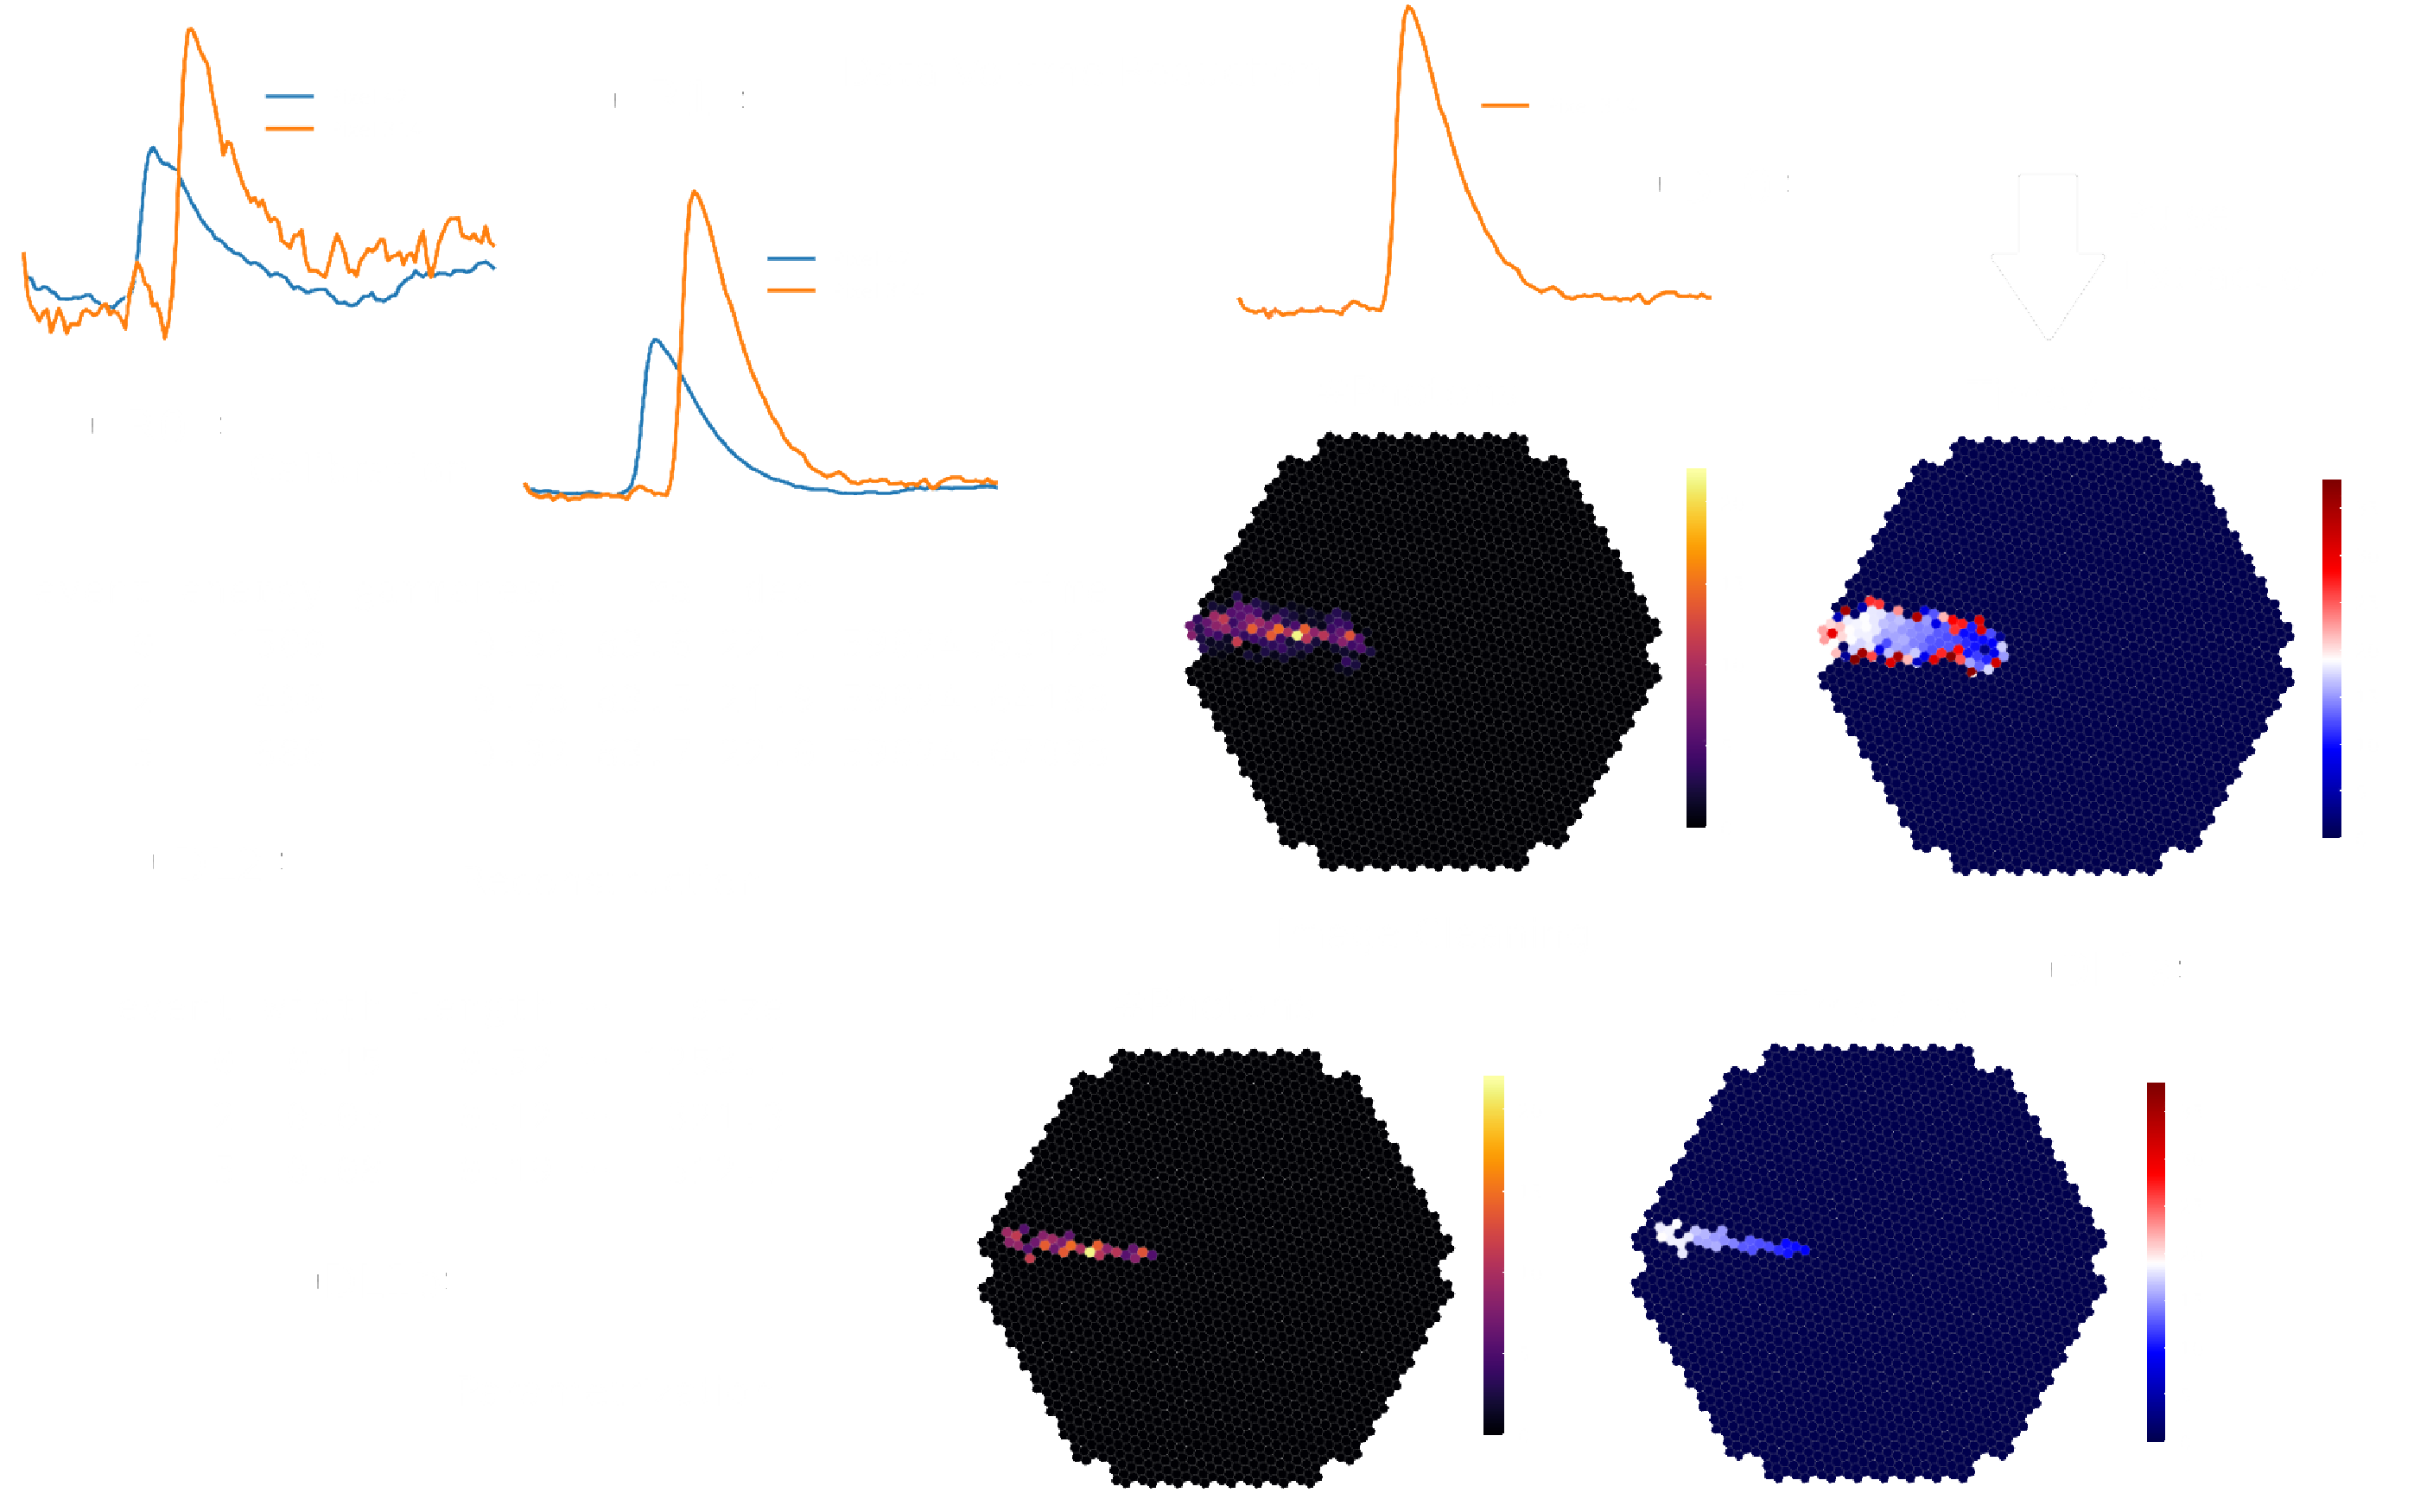
\includegraphics[height=0.9\textheight]{graphics/ctapipe_light.pdf}
    \vspace{-0.25cm}
    \footnote{\textcolor{white!85!black}{Adapted from J.~Hackfeld and M.~Linhoff}}
    }
    {% use light theme
    \centering
    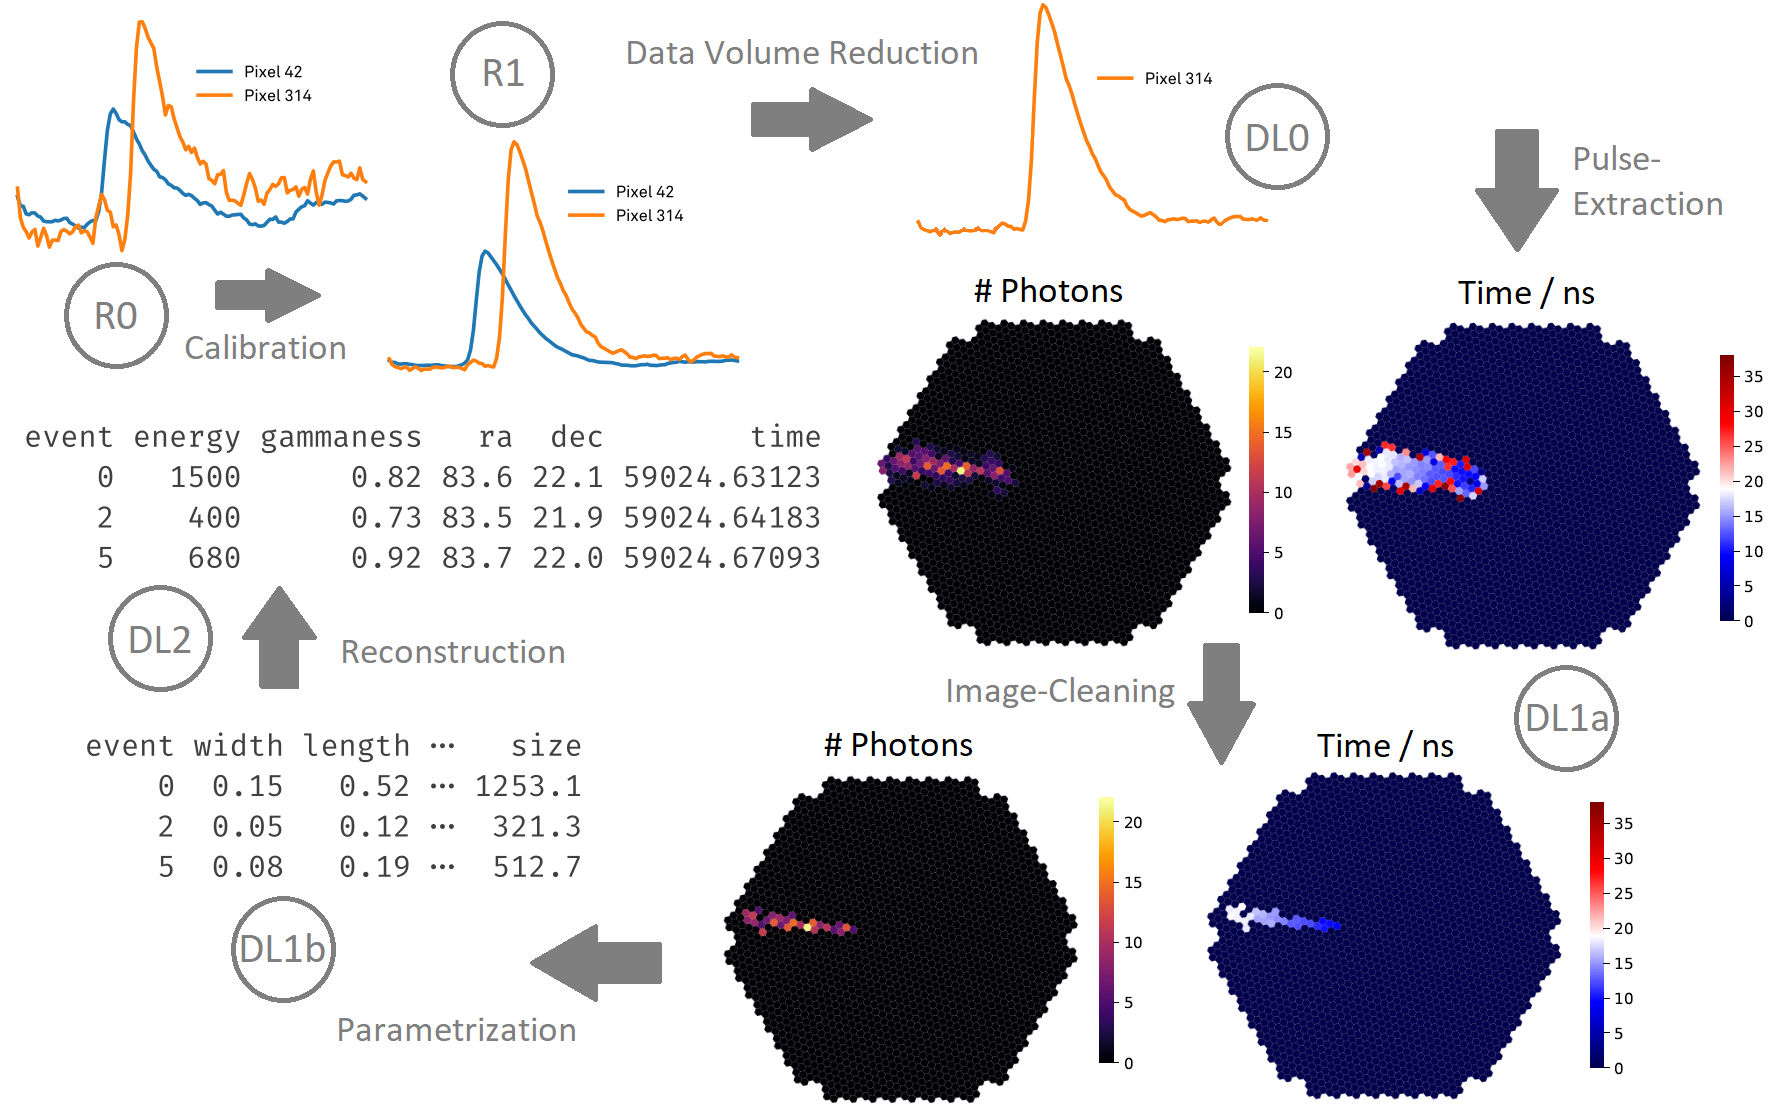
\includegraphics[height=0.9\textheight]{graphics/ctapipe.png}
    \vspace{-0.25cm}
    \footnote{\textcolor{darkgray!85!black}{Adapted from J.~Hackfeld and M.~Linhoff}}
    }
\end{frame}

\begin{frame}
    \ifthenelse{\equal{\theme}{\string 1}}
    {% use dark theme
    \centering
    \includegraphics[width=\textwidth]{build/tikz/data_pipeline_dark.pdf}
    }
    {% use light theme
    \centering
    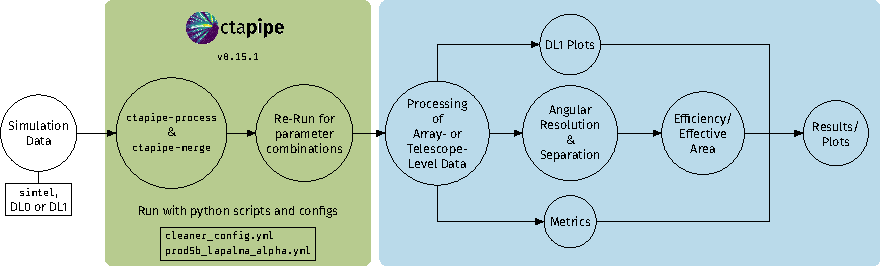
\includegraphics[width=\textwidth]{build/tikz/data_pipeline.pdf}
    }
\end{frame}

\subsection{Cleaning Algorithms}%
\label{sub:Cleaning_algorithms}

\ifthenelse{\equal{\theme}{\string 1}}
    {% use dark theme
    \begin{frame}[t]{Cleaning Algorithms}
    \raisebox{10ex}{
    \begin{overlayarea}{0.36\textwidth}{3.5cm}
      \only<1>{
      \begin{itemize}
        \setlength\itemsep{1em}
        \item \code{white}{TailcutsImageCleaner}
        \item \code{white}{MARSImageCleaner}
        \item \code{white}{FACTImageCleaner}
        \item \code{white}{TimeConstrainedImageCleaner}
      \end{itemize}
      }
      \only<2>{
      \begin{itemize}
        \setlength\itemsep{1em}
        \item \code{white}{TailcutsImageCleaner}
        \item \code{white!50!black}{MARSImageCleaner}
        \item \code{white!50!black}{FACTImageCleaner}
        \item \code{white!50!black}{TimeConstrainedImageCleaner}
      \end{itemize}
      }
      \only<3>{
        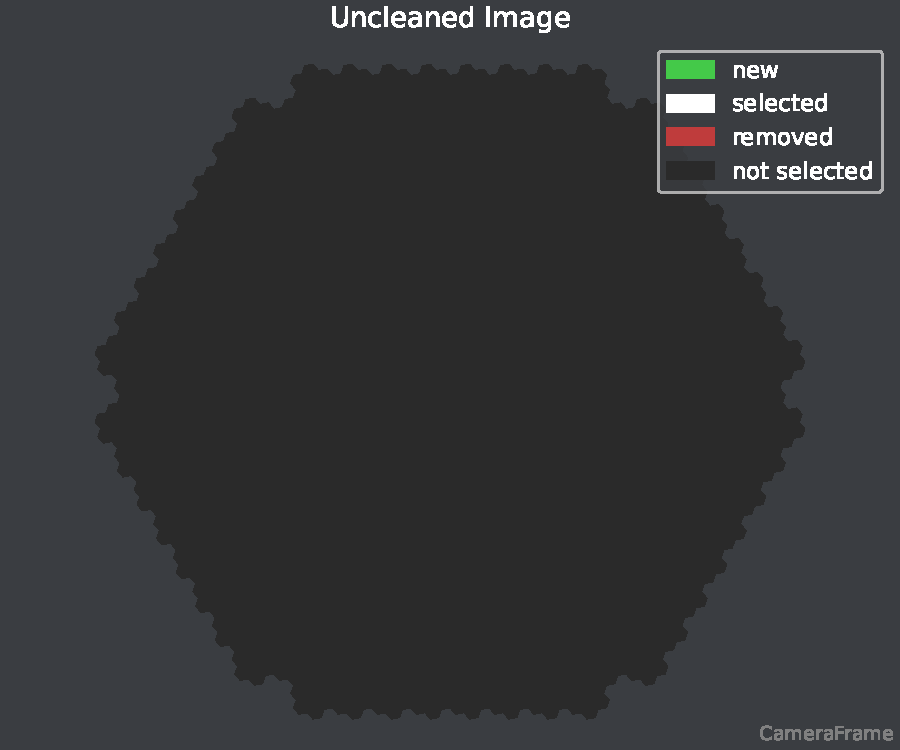
\includegraphics[width=\textwidth]{plots/cleaner_steps/dark/null_image.pdf}
      }
      \only<4>{
        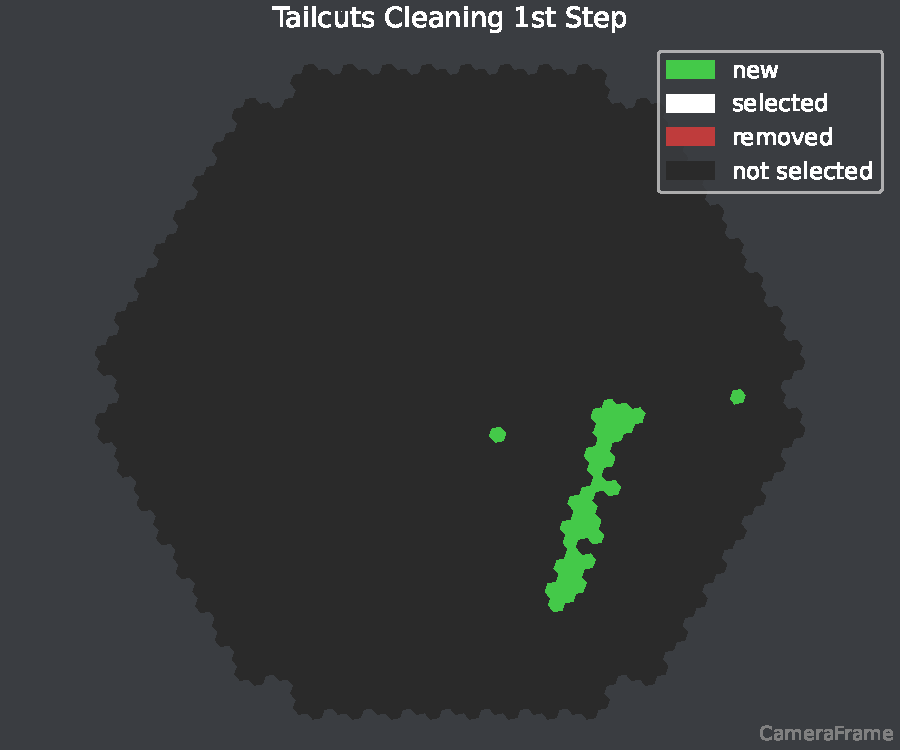
\includegraphics[width=\textwidth]{plots/cleaner_steps/dark/tail_1.pdf}
      }
      \only<5>{
        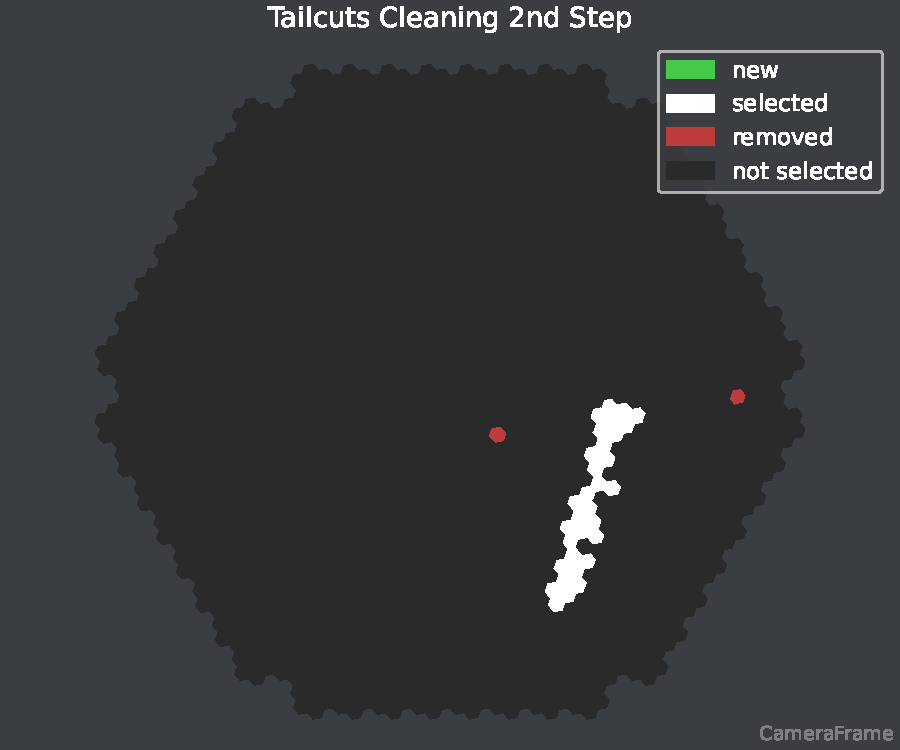
\includegraphics[width=\textwidth]{plots/cleaner_steps/dark/tail_2.pdf}
      }
      \only<6>{
      \begin{itemize}
        \setlength\itemsep{1em}
        \item \code{white!50!black}{TailcutsImageCleaner}
        \item \code{white}{MARSImageCleaner}
        \item \code{white!50!black}{FACTImageCleaner}
        \item \code{white!50!black}{TimeConstrainedImageCleaner}
      \end{itemize}
      }
      \only<7>{
        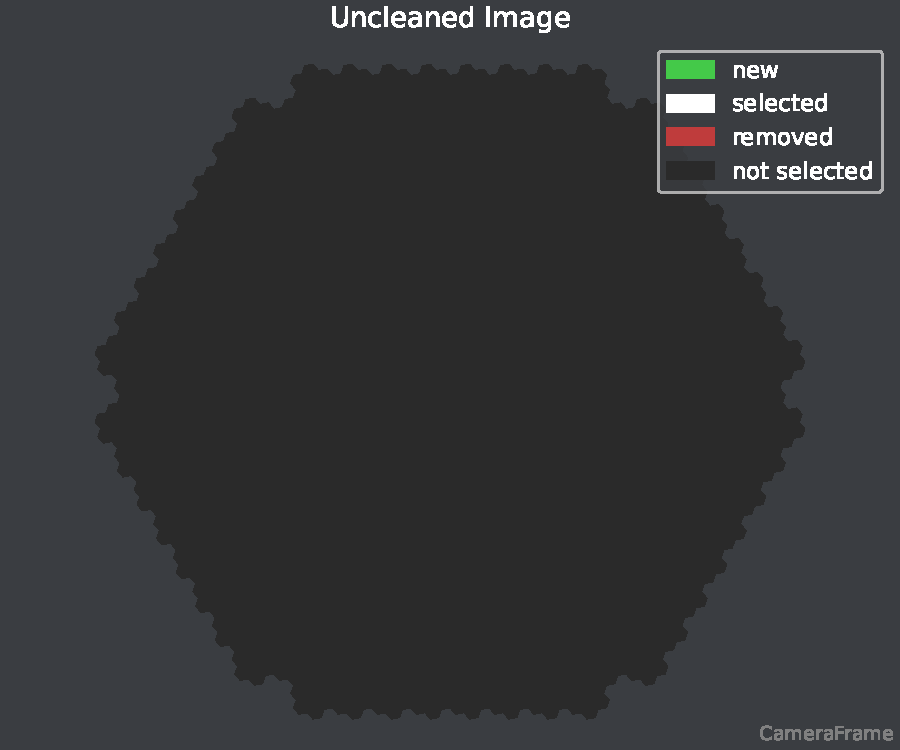
\includegraphics[width=\textwidth]{plots/cleaner_steps/dark/null_image.pdf}
      }
      \only<8>{
        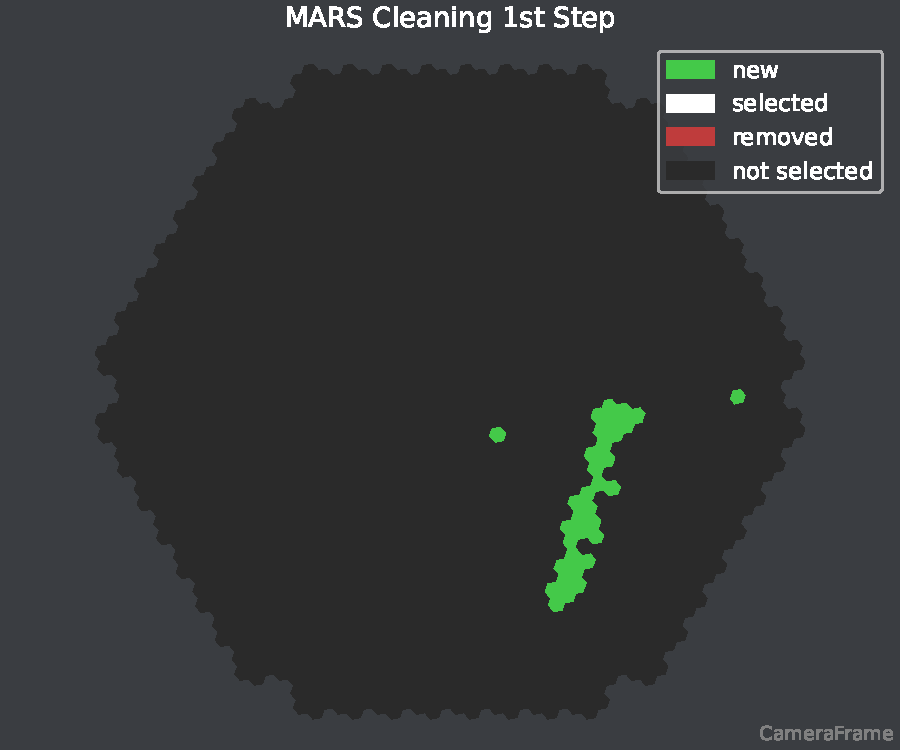
\includegraphics[width=\textwidth]{plots/cleaner_steps/dark/mars_1.pdf}
      }
      \only<9>{
        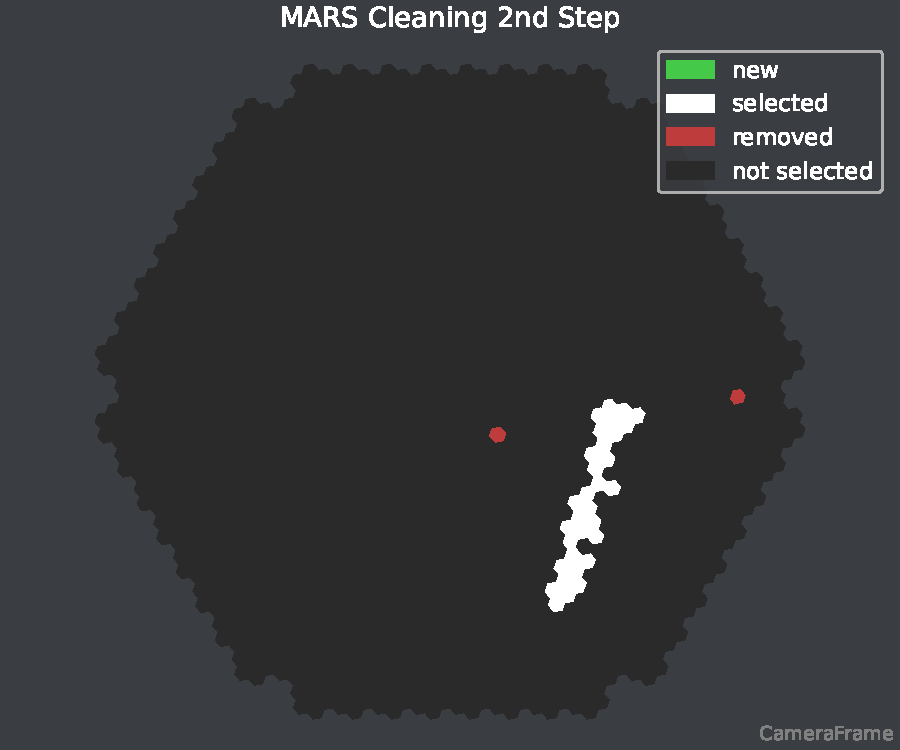
\includegraphics[width=\textwidth]{plots/cleaner_steps/dark/mars_2.pdf}
      }
      \only<10>{
        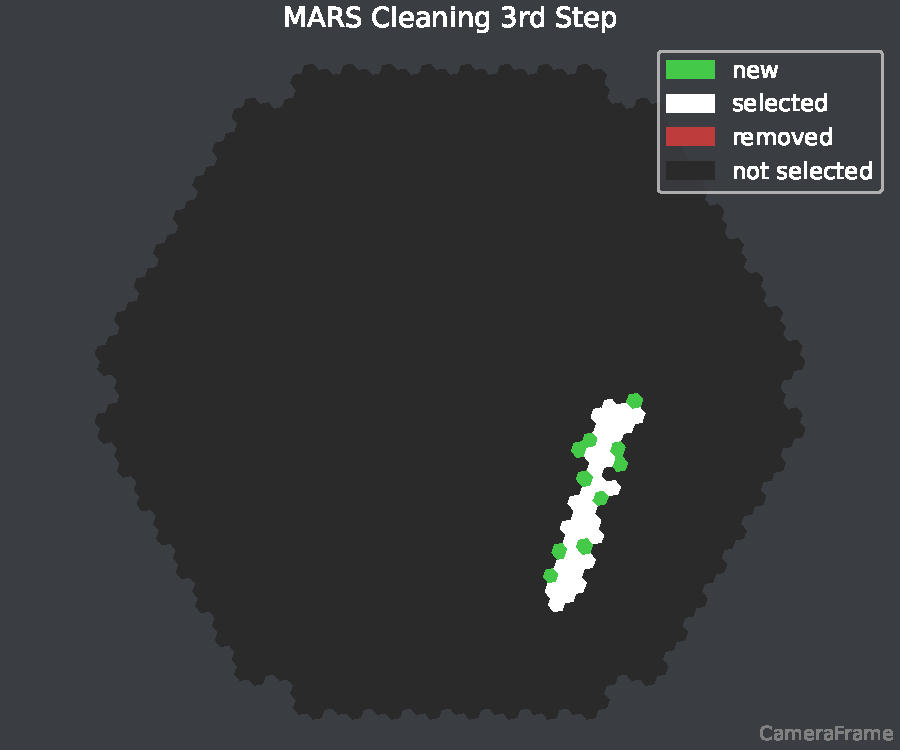
\includegraphics[width=\textwidth]{plots/cleaner_steps/dark/mars_3.pdf}
      }
      \only<11>{
      \begin{itemize}
        \setlength\itemsep{1em}
        \item \code{white!50!black}{TailcutsImageCleaner}
        \item \code{white!50!black}{MARSImageCleaner}
        \item \code{white}{FACTImageCleaner}
        \item \code{white!50!black}{TimeConstrainedImageCleaner}
      \end{itemize}
      }
      \only<12>{
        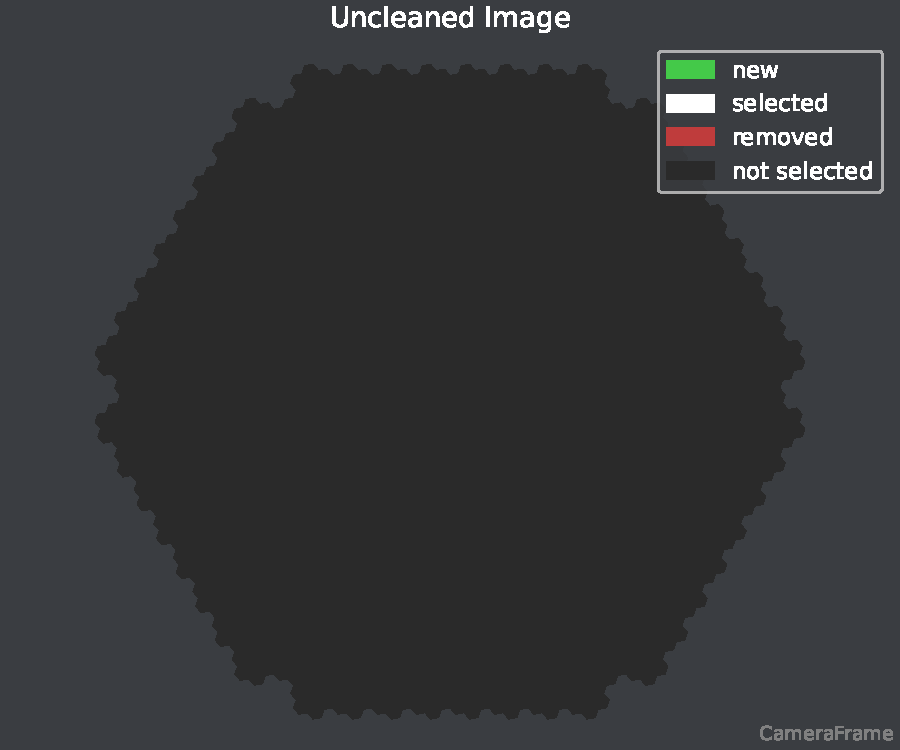
\includegraphics[width=\textwidth]{plots/cleaner_steps/dark/null_image.pdf}
      }
      \only<13>{
        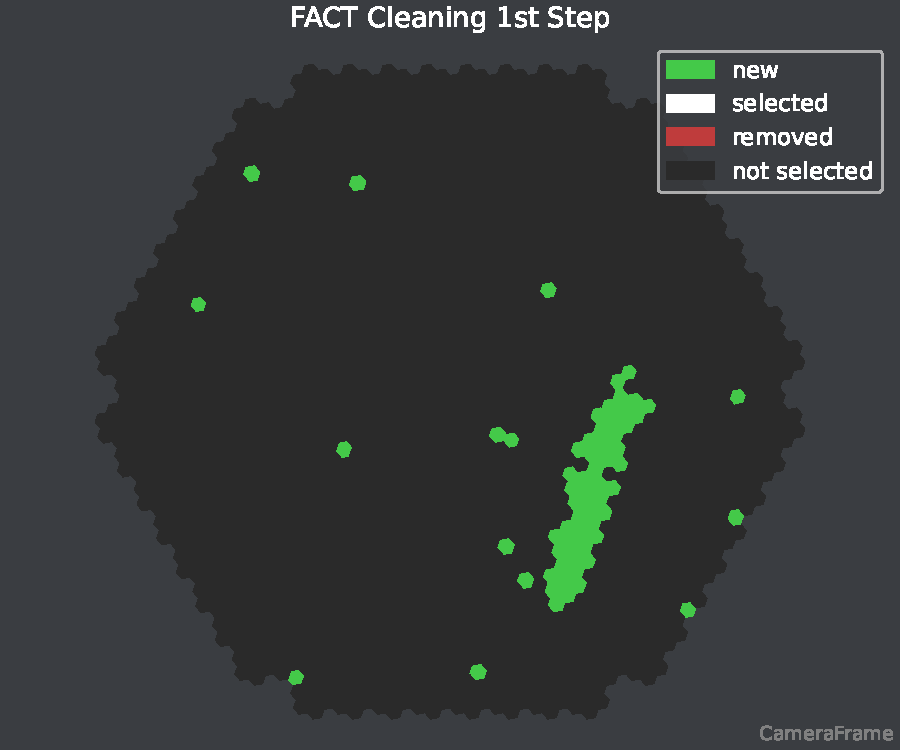
\includegraphics[width=\textwidth]{plots/cleaner_steps/dark/fact_1.pdf}
      }
      \only<14>{
        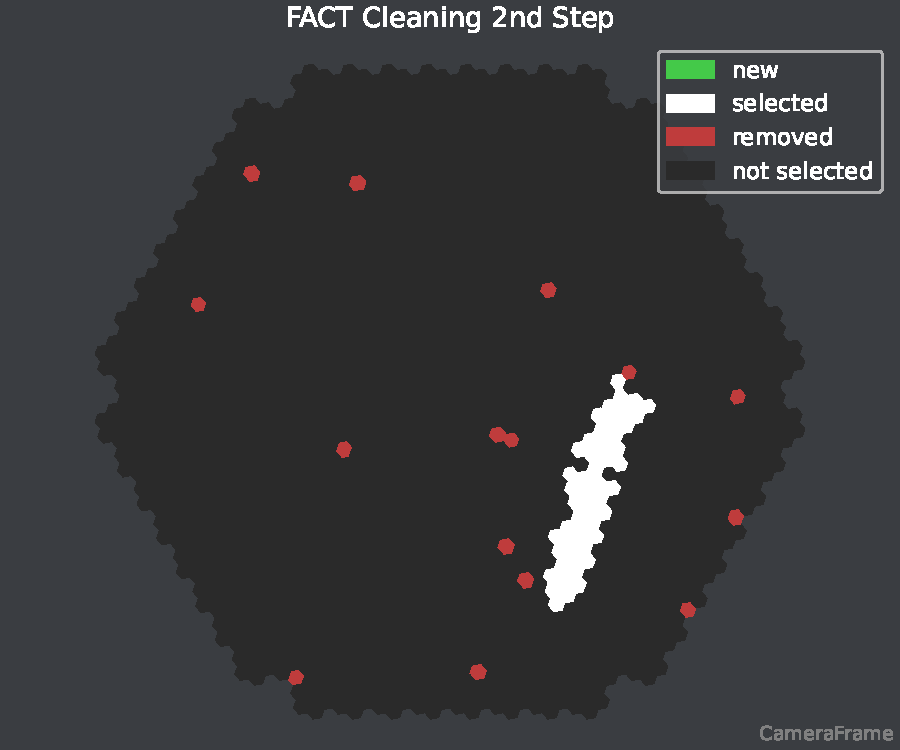
\includegraphics[width=\textwidth]{plots/cleaner_steps/dark/fact_2.pdf}
      }
      \only<15>{
        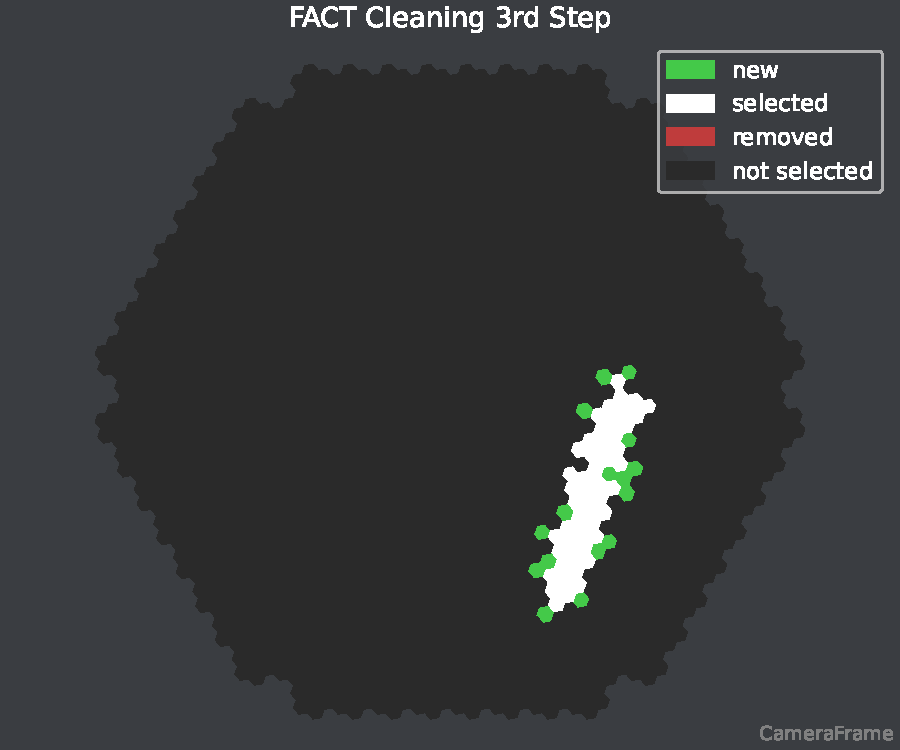
\includegraphics[width=\textwidth]{plots/cleaner_steps/dark/fact_3.pdf}
      }
      \only<16>{
        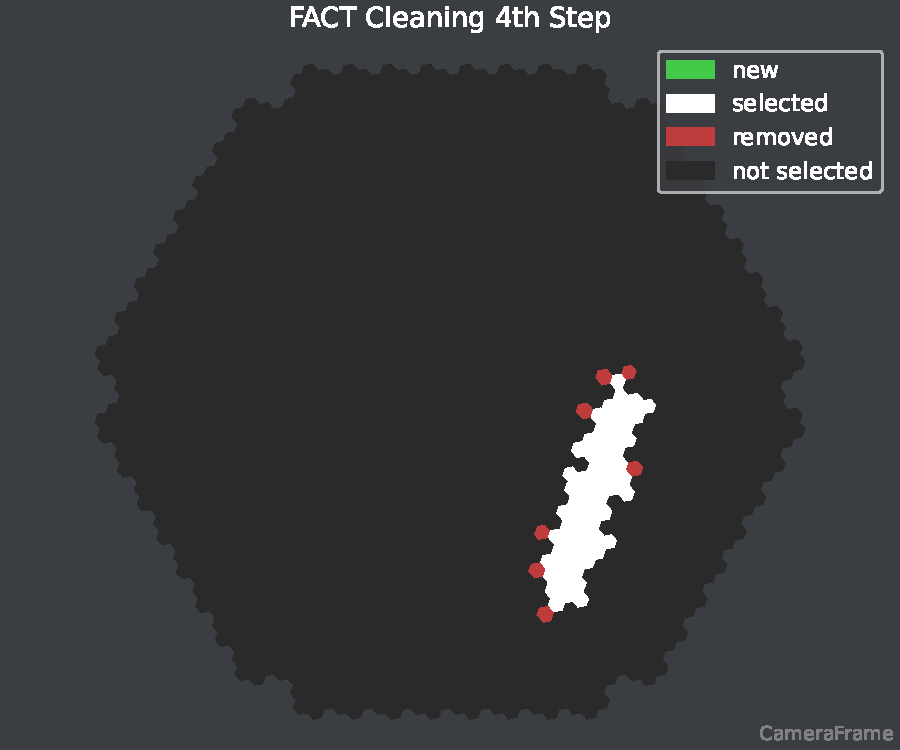
\includegraphics[width=\textwidth]{plots/cleaner_steps/dark/fact_4.pdf}
      }
      \only<17>{
        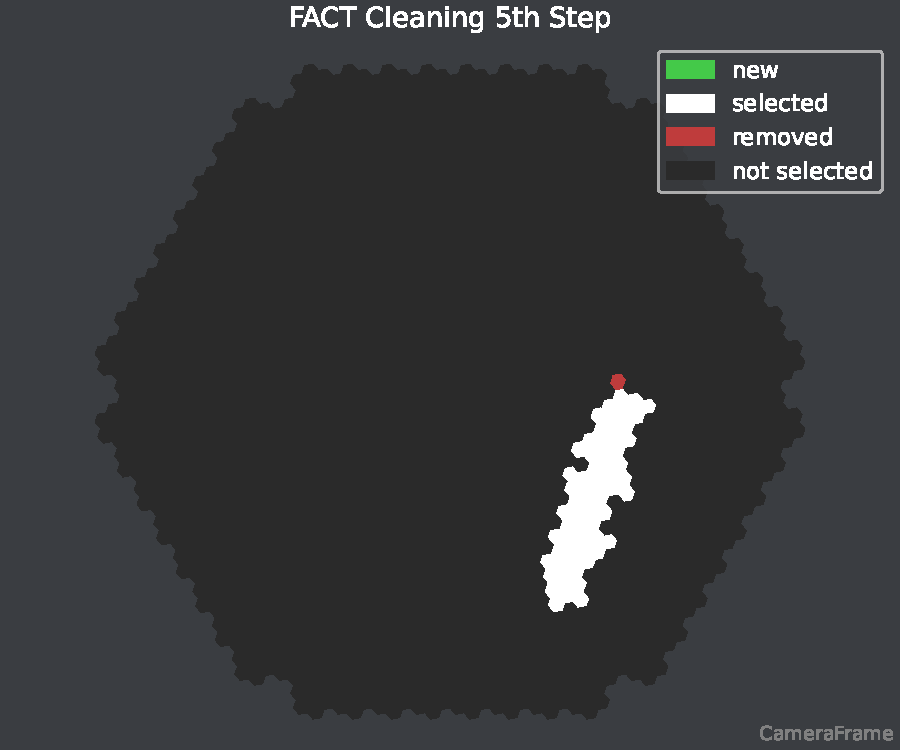
\includegraphics[width=\textwidth]{plots/cleaner_steps/dark/fact_5.pdf}
      }
      \only<18>{
        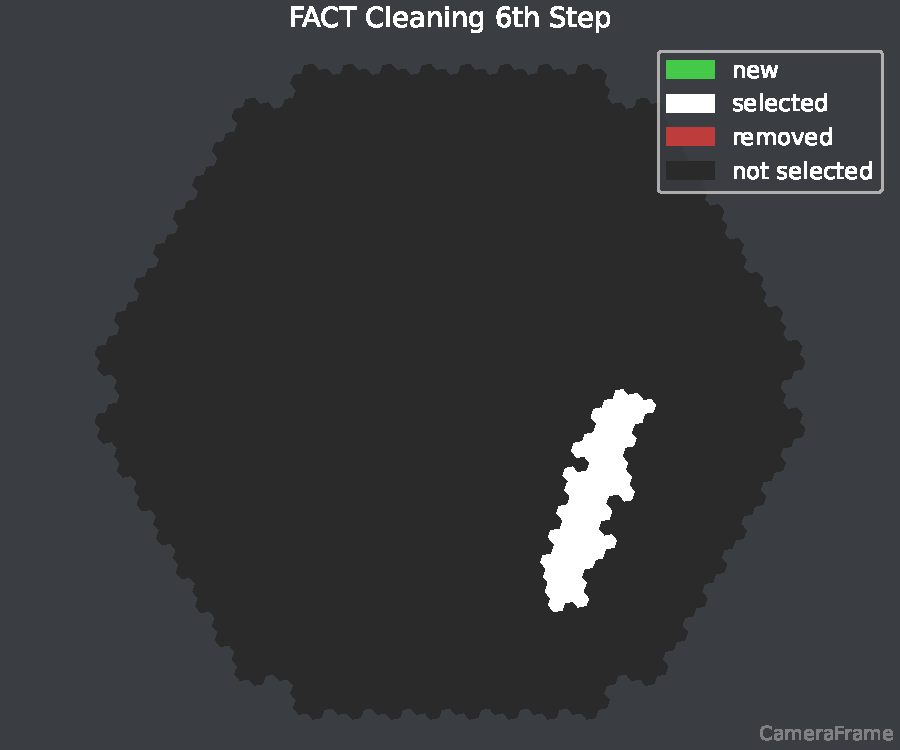
\includegraphics[width=\textwidth]{plots/cleaner_steps/dark/fact_6.pdf}
      }
      \only<19>{
      \begin{itemize}
        \setlength\itemsep{1em}
        \item \code{white!50!black}{TailcutsImageCleaner}
        \item \code{white!50!black}{MARSImageCleaner}
        \item \code{white!50!black}{FACTImageCleaner}
        \item \code{white}{TimeConstrainedImageCleaner}
      \end{itemize}
      }
      \only<20>{
        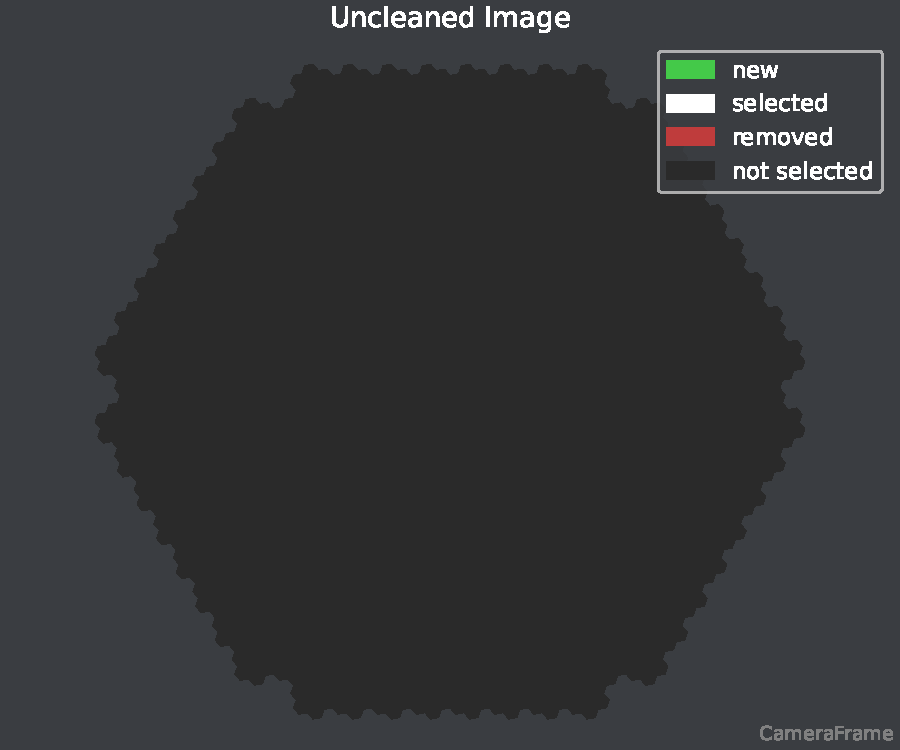
\includegraphics[width=\textwidth]{plots/cleaner_steps/dark/null_image.pdf}
      }
      \only<21>{
        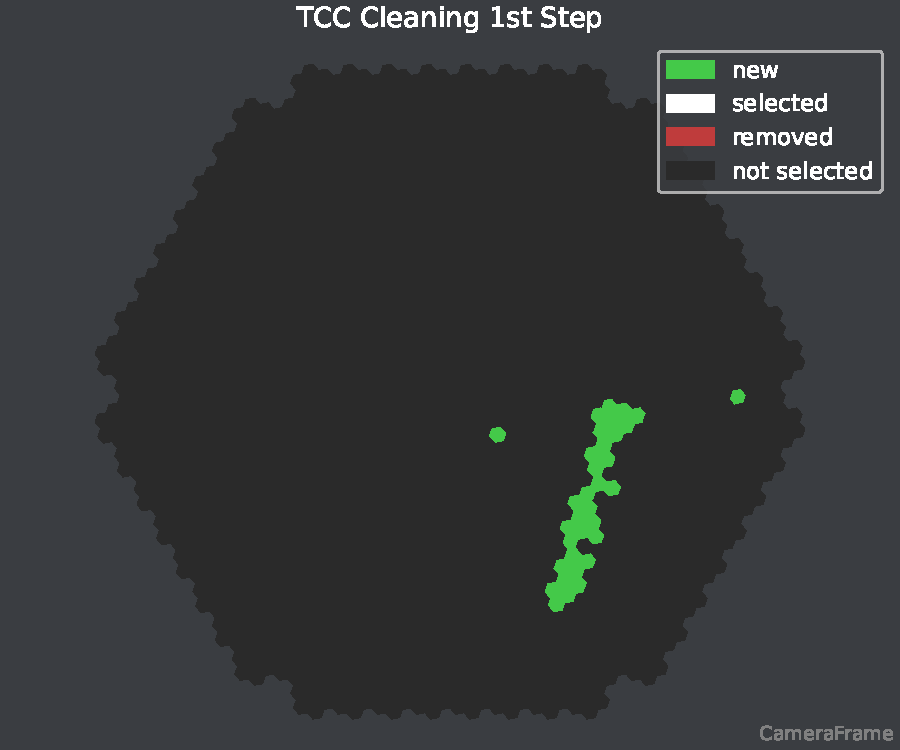
\includegraphics[width=\textwidth]{plots/cleaner_steps/dark/tcc_1.pdf}
      }
      \only<22>{
        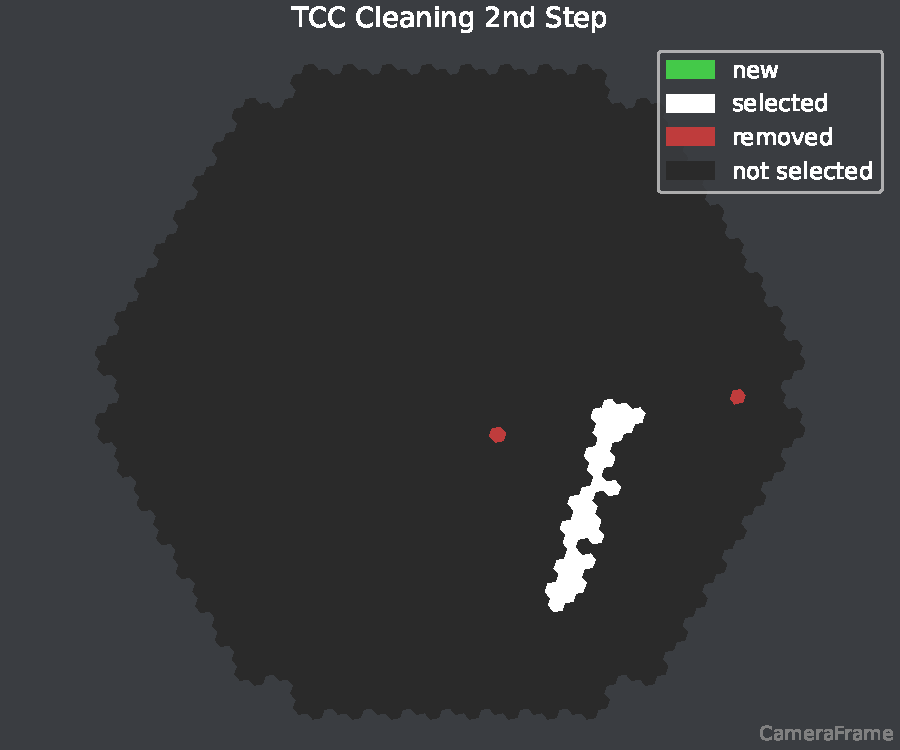
\includegraphics[width=\textwidth]{plots/cleaner_steps/dark/tcc_2.pdf}
      }
      \only<23>{
        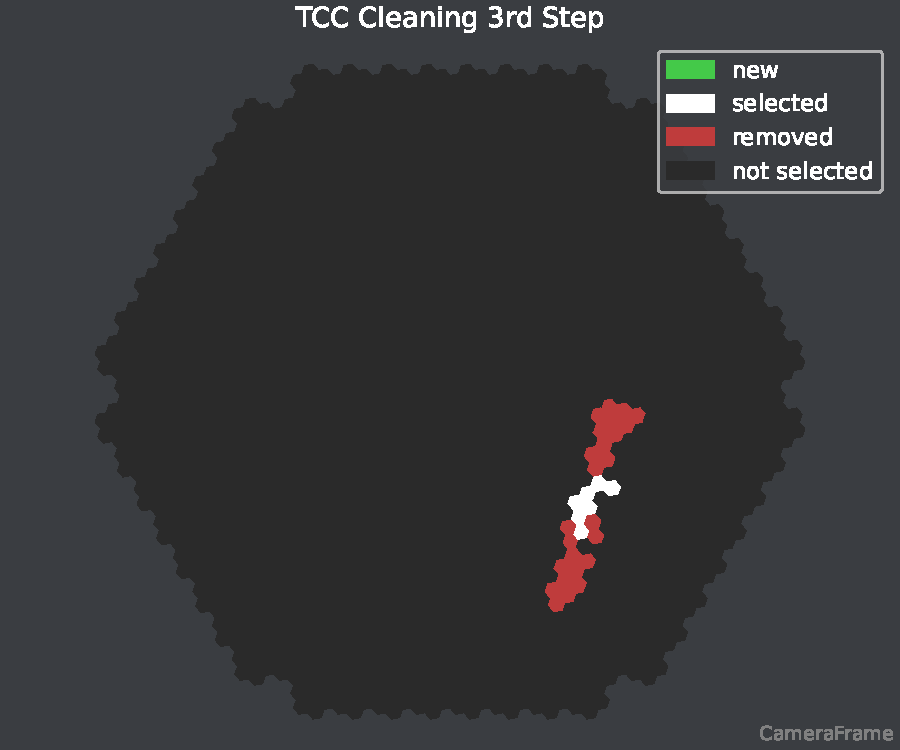
\includegraphics[width=\textwidth]{plots/cleaner_steps/dark/tcc_3.pdf}
      }
      \only<24>{
        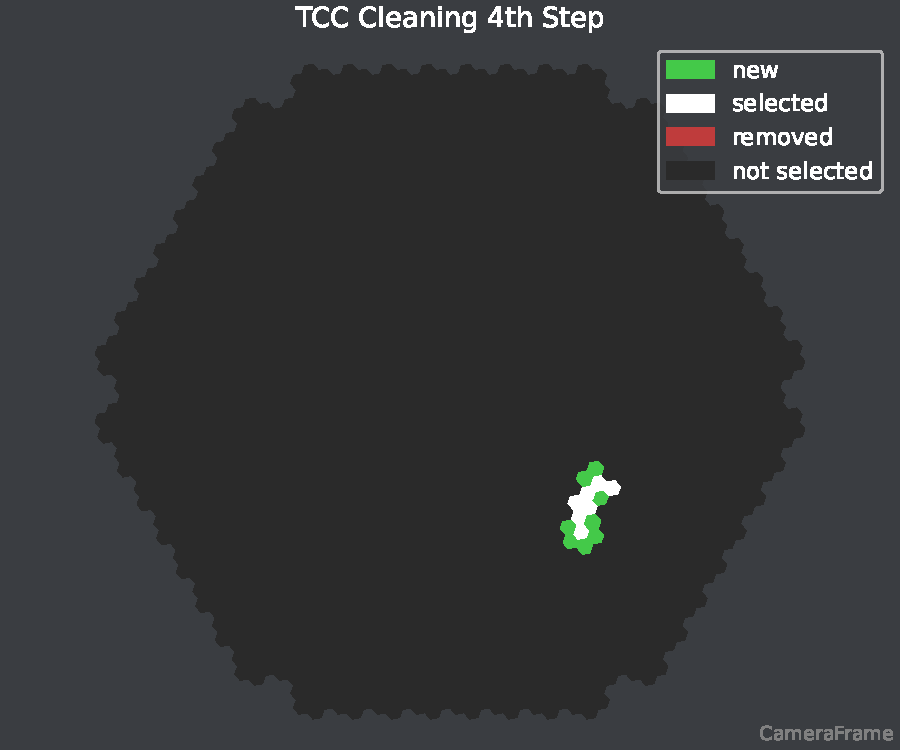
\includegraphics[width=\textwidth]{plots/cleaner_steps/dark/tcc_4.pdf}
      }
      \only<25>{
        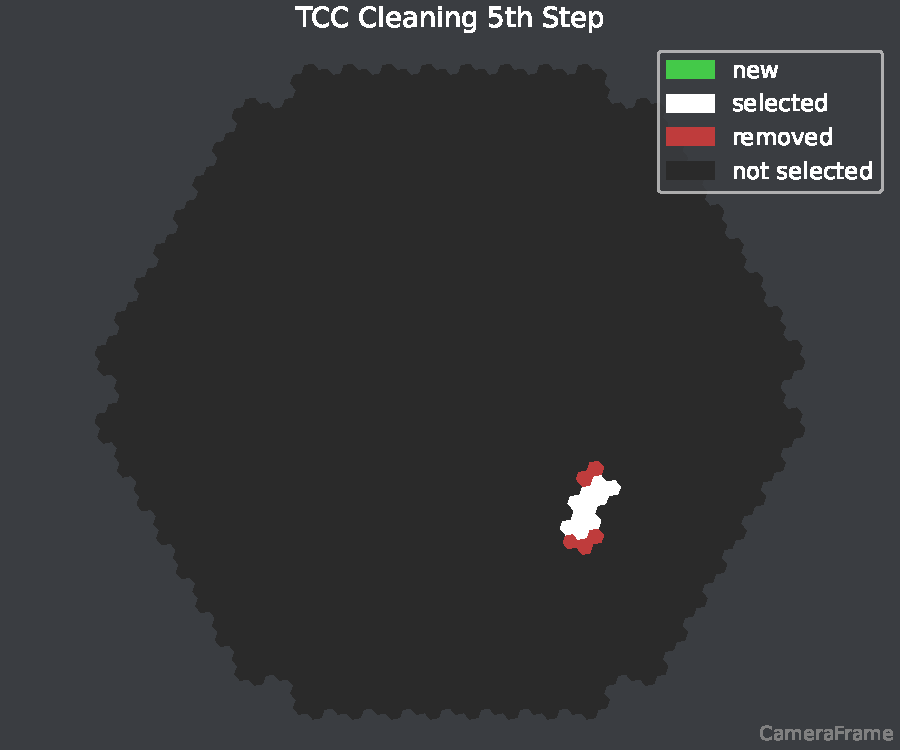
\includegraphics[width=\textwidth]{plots/cleaner_steps/dark/tcc_5.pdf}
      }
    \end{overlayarea}
    }
    \raisebox{10ex}{
    \begin{overlayarea}{0.58\textwidth}{3.5cm}
      \only<1>{
        \centering
        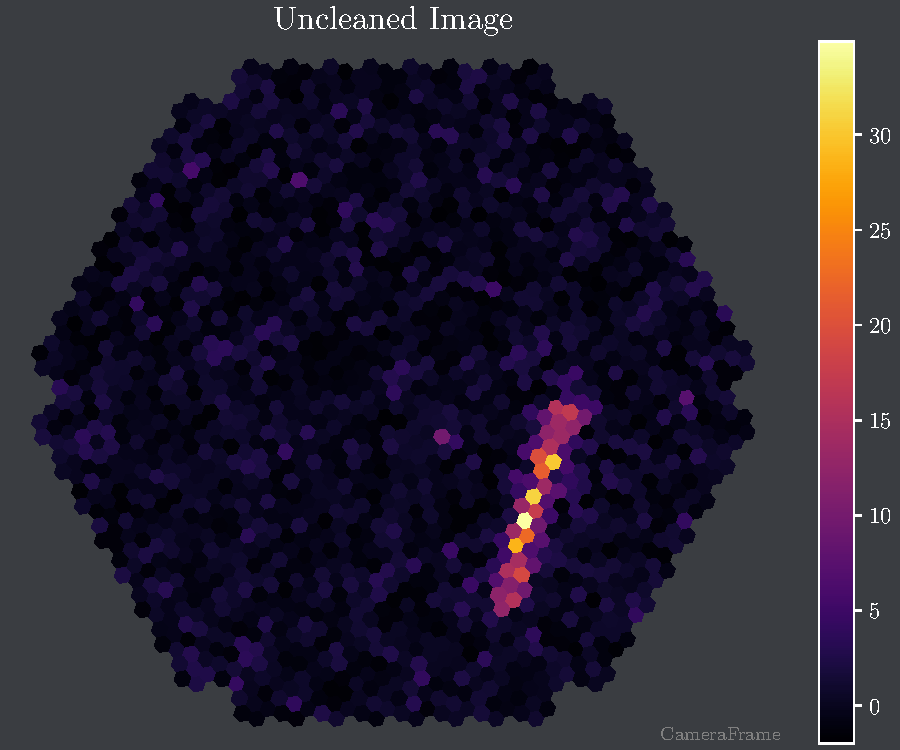
\includegraphics[width=0.65\textwidth]{plots/cleaner_steps/dark/uncleaned_image.pdf}
      }
      \only<2>{
      \begin{enumerate}%TailcutsImageCleaner
        \item Select pixels that pass the \code{white!70!black}{core threshold} (this talk: \(\SI{7}{\pe}\))
        \item Add pixels that pass the \code{white!70!black}{boundary threshold} (here: \(\SI{5}{\pe}\))
      \end{enumerate}
      }
      \only<3>{
      \begin{enumerate}%TailcutsImageCleaner
        \item \textcolor{white!50!black}{Select pixels that pass the \code{white!35!black}{core threshold} (this talk: \(\SI{7}{\pe}\))}
        \item \textcolor{white!50!black}{Add pixels that pass the \code{white!35!black}{boundary threshold} (here: \(\SI{5}{\pe}\))}
      \end{enumerate}
      }
      \only<4>{
      \begin{enumerate}%TailcutsImageCleaner
        \item Select pixels that pass the \code{white!70!black}{core threshold} (this talk: \(\SI{7}{\pe}\))
        \item \textcolor{white!50!black}{Add pixels that pass the \code{white!35!black}{boundary threshold} (here: \(\SI{5}{\pe}\))}
      \end{enumerate}
      }
      \only<5>{
      \begin{enumerate}%TailcutsImageCleaner
        \item \textcolor{white!50!black}{Select pixels that pass the \code{white!35!black}{core threshold} (this talk: \(\SI{7}{\pe}\))}
        \item Add pixels that pass the \code{white!70!black}{boundary threshold} (here: \(\SI{5}{\pe}\))
      \end{enumerate}
      }

      \only<6>{
      \begin{enumerate}%MARSImageCleaner
        \item Select pixels that pass the \code{white!70!black}{core} and \code{white!70!black}{boundary threshold}, analogous to \code{white!70!black}{TailcutsImageCleaner}
        \item Add pixels that are a neighbor of a neighbor of a core pixel, if they are above the \code{white!70!black}{boundary threshold}
      \end{enumerate}
      }
      \only<7>{
      \begin{enumerate}%MARSImageCleaner
        \item \textcolor{white!50!black}{Select pixels that pass the \code{white!35!black}{core} and \code{white!35!black}{boundary threshold}, analogous to \code{white!35!black}{TailcutsImageCleaner}}
        \item \textcolor{white!50!black}{Add pixels that are a neighbor of a neighbor of a core pixel, if they are above the \code{white!35!black}{boundary threshold}}
      \end{enumerate}
      }
      \only<8-9>{
      \begin{enumerate}%MARSImageCleaner
        \item Select pixels that pass the \code{white!70!black}{core} and \code{white!70!black}{boundary threshold}, analogous to \code{white!70!black}{TailcutsImageCleaner}
        \item \textcolor{white!50!black}{Add pixels that are a neighbor of a neighbor of a core pixel, if they are above the \code{white!35!black}{boundary threshold}}
      \end{enumerate}
      }
      \only<10>{
      \begin{enumerate}%MARSImageCleaner
        \item \textcolor{white!50!black}{Select pixels that pass the \code{white!35!black}{core} and \code{white!35!black}{boundary threshold}, analogous to \code{white!35!black}{TailcutsImageCleaner}}
        \item Add pixels that are a neighbor of a neighbor of a core pixel, if they are above the \code{white!70!black}{boundary threshold}
      \end{enumerate}
      }
      \only<11>{
      \begin{enumerate}%FACTImageCleaner
        \item Find all pixels that contain more photons than the \code{white!70!black}{core threshold} (this talk: \(\SI{4}{\pe}\))
        \item Remove pixels with less than \(N\) neighbors (this talk: \(N=2\))
        \item Add remaining neighbors that are above the \code{white!70!black}{boundary threshold} (this talk: \(\SI{2}{\pe}\))
        \item Remove pixels that have less than \(N\) neighbors, that arrive within a given timeframe (here: \SI{5}{\nano\second})
        \item Remove pixels that have less than \(N\) neighbors
        \item Remove pixels that have less than \(N\) neighbors, arriving within a given timeframe (same as in step 4)
      \end{enumerate}
      }
      \only<12>{
      \begin{enumerate}%FACTImageCleaner
        \item \textcolor{white!50!black}{Find all pixels that contain more photons than the \code{white!35!black}{core threshold} (this talk: \(\SI{4}{\pe}\))}
        \item \textcolor{white!50!black}{Remove pixels with less than \(N\) neighbors (this talk: \(N=2\))}
        \item \textcolor{white!50!black}{Add remaining neighbors that are above the \code{white!35!black}{boundary threshold} (this talk: \(\SI{2}{\pe}\))}
        \item \textcolor{white!50!black}{Remove pixels that have less than \(N\) neighbors, that arrive within a given timeframe (here: \SI{5}{\nano\second})}
        \item \textcolor{white!50!black}{Remove pixels that have less than \(N\) neighbors}
        \item \textcolor{white!50!black}{Remove pixels that have less than \(N\) neighbors, arriving within a given timeframe (same as in step 4)}
      \end{enumerate}
      }
      \only<13>{
      \begin{enumerate}%FACTImageCleaner
        \item Find all pixels that contain more photons than the \code{white!70!black}{core threshold} (this talk: \(\SI{4}{\pe}\))
        \item \textcolor{white!50!black}{Remove pixels with less than \(N\) neighbors (this talk: \(N=2\))}
        \item \textcolor{white!50!black}{Add remaining neighbors that are above the \code{white!35!black}{boundary threshold} (this talk: \(\SI{2}{\pe}\))}
        \item \textcolor{white!50!black}{Remove pixels that have less than \(N\) neighbors, that arrive within a given timeframe (here: \SI{5}{\nano\second})}
        \item \textcolor{white!50!black}{Remove pixels that have less than \(N\) neighbors}
        \item \textcolor{white!50!black}{Remove pixels that have less than \(N\) neighbors, arriving within a given timeframe (same as in step 4)}
      \end{enumerate}
      }
      \only<14>{
      \begin{enumerate}%FACTImageCleaner
        \item \textcolor{white!50!black}{Find all pixels that contain more photons than the \code{white!35!black}{core threshold} (this talk: \(\SI{4}{\pe}\))}
        \item Remove pixels with less than \(N\) neighbors (this talk: \(N=2\))
        \item \textcolor{white!50!black}{Add remaining neighbors that are above the \code{white!35!black}{boundary threshold} (this talk: \(\SI{2}{\pe}\))}
        \item \textcolor{white!50!black}{Remove pixels that have less than \(N\) neighbors, that arrive within a given timeframe (here: \SI{5}{\nano\second})}
        \item \textcolor{white!50!black}{Remove pixels that have less than \(N\) neighbors}
        \item \textcolor{white!50!black}{Remove pixels that have less than \(N\) neighbors, arriving within a given timeframe (same as in step 4)}
      \end{enumerate}
      }
      \only<15>{
      \begin{enumerate}%FACTImageCleaner
        \item \textcolor{white!50!black}{Find all pixels that contain more photons than the \code{white!35!black}{core threshold} (this talk: \(\SI{4}{\pe}\))}
        \item \textcolor{white!50!black}{Remove pixels with less than \(N\) neighbors (this talk: \(N=2\))}
        \item Add remaining neighbors that are above the \code{white!70!black}{boundary threshold} (this talk: \(\SI{2}{\pe}\))
        \item \textcolor{white!50!black}{Remove pixels that have less than \(N\) neighbors, that arrive within a given timeframe (here: \SI{5}{\nano\second})}
        \item \textcolor{white!50!black}{Remove pixels that have less than \(N\) neighbors}
        \item \textcolor{white!50!black}{Remove pixels that have less than \(N\) neighbors, arriving within a given timeframe (same as in step 4)}
      \end{enumerate}
      }
      \only<16>{
      \begin{enumerate}%FACTImageCleaner
        \item \textcolor{white!50!black}{Find all pixels that contain more photons than the \code{white!35!black}{core threshold} (this talk: \(\SI{4}{\pe}\))}
        \item \textcolor{white!50!black}{Remove pixels with less than \(N\) neighbors (this talk: \(N=2\))}
        \item \textcolor{white!50!black}{Add remaining neighbors that are above the \code{white!35!black}{boundary threshold} (this talk: \(\SI{2}{\pe}\))}
        \item Remove pixels that have less than \(N\) neighbors, that arrive within a given timeframe (here: \SI{5}{\nano\second})
        \item \textcolor{white!50!black}{Remove pixels that have less than \(N\) neighbors}
        \item \textcolor{white!50!black}{Remove pixels that have less than \(N\) neighbors, arriving within a given timeframe (same as in step 4)}
      \end{enumerate}
      }
      \only<17>{
      \begin{enumerate}%FACTImageCleaner
        \item \textcolor{white!50!black}{Find all pixels that contain more photons than the \code{white!35!black}{core threshold} (this talk: \(\SI{4}{\pe}\))}
        \item \textcolor{white!50!black}{Remove pixels with less than \(N\) neighbors (this talk: \(N=2\))}
        \item \textcolor{white!50!black}{Add remaining neighbors that are above the \code{white!35!black}{boundary threshold} (this talk: \(\SI{2}{\pe}\))}
        \item \textcolor{white!50!black}{Remove pixels that have less than \(N\) neighbors, that arrive within a given timeframe (here: \SI{5}{\nano\second})}
        \item Remove pixels that have less than \(N\) neighbors
        \item \textcolor{white!50!black}{Remove pixels that have less than \(N\) neighbors, arriving within a given timeframe (same as in step 4)}
      \end{enumerate}
      }
      \only<18>{
      \begin{enumerate}%FACTImageCleaner
        \item \textcolor{white!50!black}{Find all pixels that contain more photons than the \code{white!35!black}{core threshold} (this talk: \(\SI{4}{\pe}\))}
        \item \textcolor{white!50!black}{Remove pixels with less than \(N\) neighbors (this talk: \(N=2\))}
        \item \textcolor{white!50!black}{Add remaining neighbors that are above the \code{white!35!black}{boundary threshold} (this talk: \(\SI{2}{\pe}\))}
        \item \textcolor{white!50!black}{Remove pixels that have less than \(N\) neighbors, that arrive within a given timeframe (here: \SI{5}{\nano\second})}
        \item \textcolor{white!50!black}{Remove pixels that have less than \(N\) neighbors}
        \item Remove pixels that have less than \(N\) neighbors, arriving within the given timeframe (same as in step 4)
      \end{enumerate}
      }
      \only<19>{
      \begin{enumerate}%TimeConstrainedImageCleaner
        \item Find all core pixels above the \code{white!70!black}{core threshold} (this talk: \(\SI{7}{\pe}\))
        \item Remove pixels with less than \(N\) neighbors (this talk: \(N=1\))
        \item Keep all pixels that arrive within a time limit of the average arrival time (\code{white!70!black}{time_limit_core}: \SI{4.5}{\nano\second})
        \item Find all neighboring pixels above the \code{white!70!black}{boundary threshold} (this talk: \(\SI{5}{\pe}\))
        \item Remove all pixels with less than \(N\) neighbors arriving within a given timeframe (\code{white!70!black}{time_limit_boundary}: \SI{1.5}{\nano\second})
      \end{enumerate}
      }
      \only<20>{
      \begin{enumerate}%TimeConstrainedImageCleaner
        \item \textcolor{white!50!black}{Find all core pixels above the \code{white!35!black}{core threshold} (this talk: \(\SI{7}{\pe}\))}
        \item \textcolor{white!50!black}{Remove pixels with less than \(N\) neighbors (this talk: \(N=1\))}
        \item \textcolor{white!50!black}{Keep all pixels that arrive within a time limit of the average arrival time (\code{white!35!black}{time_limit_core}: \SI{4.5}{\nano\second})}
        \item \textcolor{white!50!black}{Find all neighboring pixels above the \code{white!35!black}{boundary threshold} (this talk: \(\SI{5}{\pe}\))}
        \item \textcolor{white!50!black}{Remove all pixels with less than \(N\) neighbors arriving within a given timeframe (\code{white!35!black}{time_limit_boundary}: \SI{1.5}{\nano\second})}
      \end{enumerate}
      }
      \only<21>{
      \begin{enumerate}%TimeConstrainedImageCleaner
        \item Find all core pixels above the \code{white!70!black}{core threshold} (this talk: \(\SI{7}{\pe}\))
        \item \textcolor{white!50!black}{Remove pixels with less than \(N\) neighbors (this talk: \(N=1\))}
        \item \textcolor{white!50!black}{Keep all pixels that arrive within a time limit of the average arrival time (\code{white!35!black}{time_limit_core}: \SI{4.5}{\nano\second})}
        \item \textcolor{white!50!black}{Find all neighboring pixels above the \code{white!35!black}{boundary threshold} (this talk: \(\SI{5}{\pe}\))}
        \item \textcolor{white!50!black}{Remove all pixels with less than \(N\) neighbors arriving within a given timeframe (\code{white!35!black}{time_limit_boundary}: \SI{1.5}{\nano\second})}
      \end{enumerate}
      }
      \only<22>{
      \begin{enumerate}%TimeConstrainedImageCleaner
        \item \textcolor{white!50!black}{Find all core pixels above the \code{white!35!black}{core threshold} (this talk: \(\SI{7}{\pe}\))}
        \item Remove pixels with less than \(N\) neighbors (this talk: \(N=1\))
        \item \textcolor{white!50!black}{Keep all pixels that arrive within a time limit of the average arrival time (\code{white!35!black}{time_limit_core}: \SI{4.5}{\nano\second})}
        \item \textcolor{white!50!black}{Find all neighboring pixels above the \code{white!35!black}{boundary threshold} (this talk: \(\SI{5}{\pe}\))}
        \item \textcolor{white!50!black}{Remove all pixels with less than \(N\) neighbors arriving within a given timeframe (\code{white!35!black}{time_limit_boundary}: \SI{1.5}{\nano\second})}
      \end{enumerate}
      }
      \only<23>{
      \begin{enumerate}%TimeConstrainedImageCleaner
        \item \textcolor{white!50!black}{Find all core pixels above the \code{white!35!black}{core threshold} (this talk: \(\SI{7}{\pe}\))}
        \item \textcolor{white!50!black}{Remove pixels with less than \(N\) neighbors (this talk: \(N=1\))}
        \item Keep all pixels that arrive within a time limit of the average arrival time (\code{white!70!black}{time_limit_core}: \SI{4.5}{\nano\second})
        \item \textcolor{white!50!black}{Find all neighboring pixels above the \code{white!35!black}{boundary threshold} (this talk: \(\SI{5}{\pe}\))}
        \item \textcolor{white!50!black}{Remove all pixels with less than \(N\) neighbors arriving within a given timeframe (\code{white!35!black}{time_limit_boundary}: \SI{1.5}{\nano\second})}
      \end{enumerate}
      }
      \only<24>{
      \begin{enumerate}%TimeConstrainedImageCleaner
        \item \textcolor{white!50!black}{Find all core pixels above the \code{white!35!black}{core threshold} (this talk: \(\SI{7}{\pe}\))}
        \item \textcolor{white!50!black}{Remove pixels with less than \(N\) neighbors (this talk: \(N=1\))}
        \item \textcolor{white!50!black}{Keep all pixels that arrive within a time limit of the average arrival time (\code{white!35!black}{time_limit_core}: \SI{4.5}{\nano\second})}
        \item Find all neighboring pixels above the \code{white!70!black}{boundary threshold} (this talk: \(\SI{5}{\pe}\))
        \item \textcolor{white!50!black}{Remove all pixels with less than \(N\) neighbors arriving within a given timeframe (\code{white!35!black}{time_limit_boundary}: \SI{1.5}{\nano\second})}
      \end{enumerate}
      }
      \only<25>{
      \begin{enumerate}%TimeConstrainedImageCleaner
        \item \textcolor{white!50!black}{Find all core pixels above the \code{white!35!black}{core threshold} (this talk: \(\SI{7}{\pe}\))}
        \item \textcolor{white!50!black}{Remove pixels with less than \(N\) neighbors (this talk: \(N=1\))}
        \item \textcolor{white!50!black}{Keep all pixels that arrive within a time limit of the average arrival time (\code{white!35!black}{time_limit_core}: \SI{4.5}{\nano\second})}
        \item \textcolor{white!50!black}{Find all neighboring pixels above the \code{white!35!black}{boundary threshold} (this talk: \(\SI{5}{\pe}\))}
        \item Remove all pixels with less than \(N\) neighbors arriving within a given timeframe (\code{white!70!black}{time_limit_boundary}: \SI{1.5}{\nano\second})
      \end{enumerate}
      }
    \end{overlayarea}
    }
  \end{frame}
    }
    {% use light theme
    \begin{frame}[t]{Cleaning Algorithms}
    \raisebox{10ex}{
    \begin{overlayarea}{0.36\textwidth}{3.5cm}
      \only<1>{
      \begin{itemize}
        \setlength\itemsep{1em}
        \item \code{darkgray}{TailcutsImageCleaner}
        \item \code{darkgray}{MARSImageCleaner}
        \item \code{darkgray}{FACTImageCleaner}
        \item \code{darkgray}{TimeConstrainedImageCleaner}
      \end{itemize}
      }
      \only<2>{
      \begin{itemize}
        \setlength\itemsep{1em}
        \item \code{darkgray}{TailcutsImageCleaner}
        \item \code{darkgray!50!white}{MARSImageCleaner}
        \item \code{darkgray!50!white}{FACTImageCleaner}
        \item \code{darkgray!50!white}{TimeConstrainedImageCleaner}
      \end{itemize}
      }
      \only<3>{
        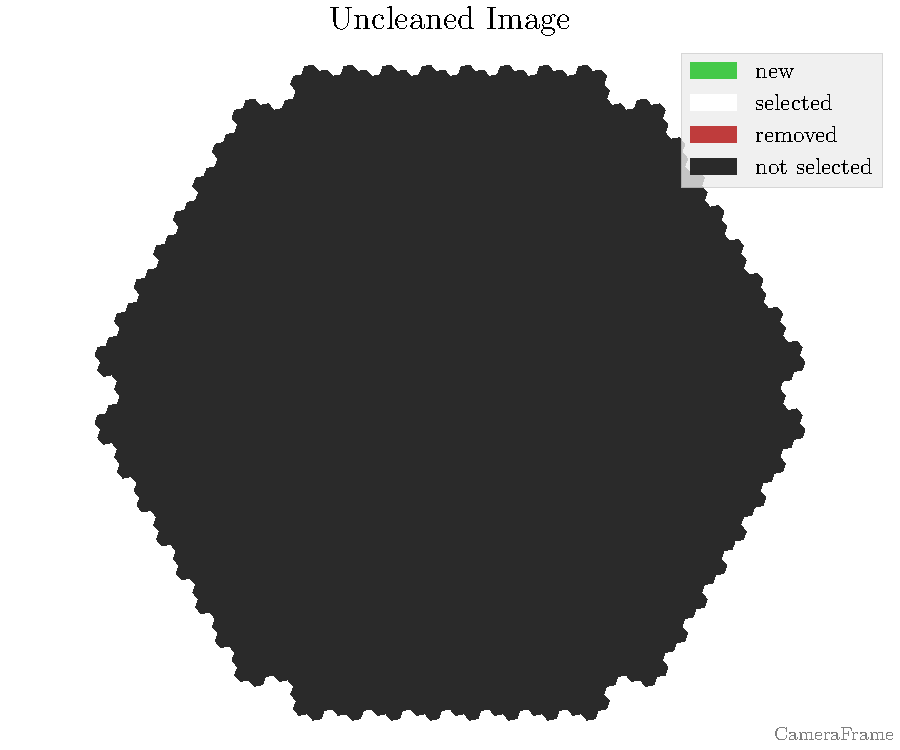
\includegraphics[width=\textwidth]{plots/cleaner_steps/light/null_image.pdf}
      }
      \only<4>{
        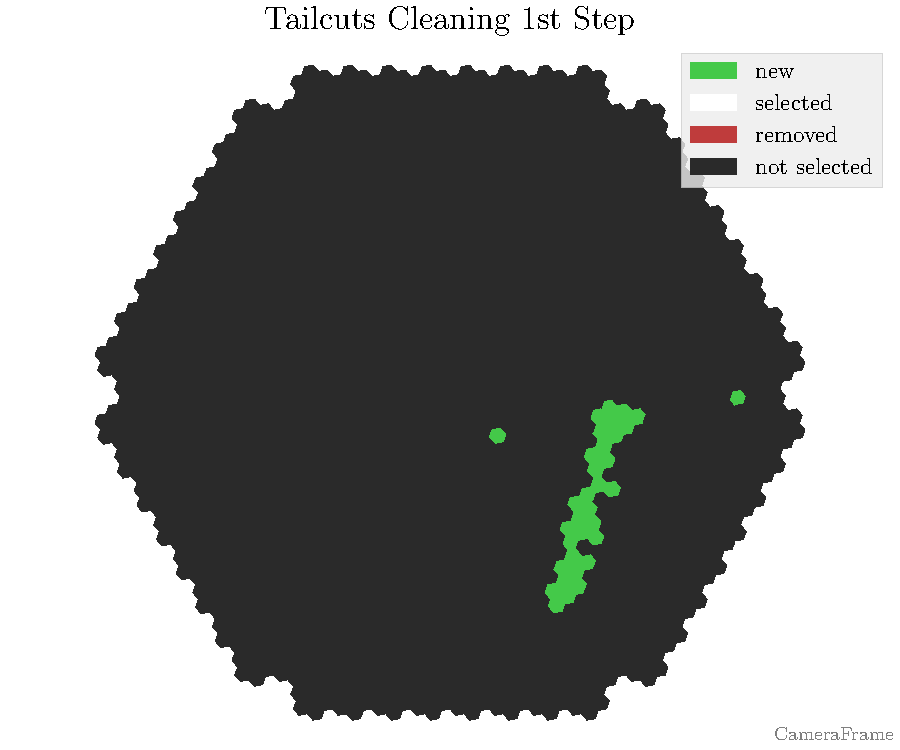
\includegraphics[width=\textwidth]{plots/cleaner_steps/light/tail_1.pdf}
      }
      \only<5>{
        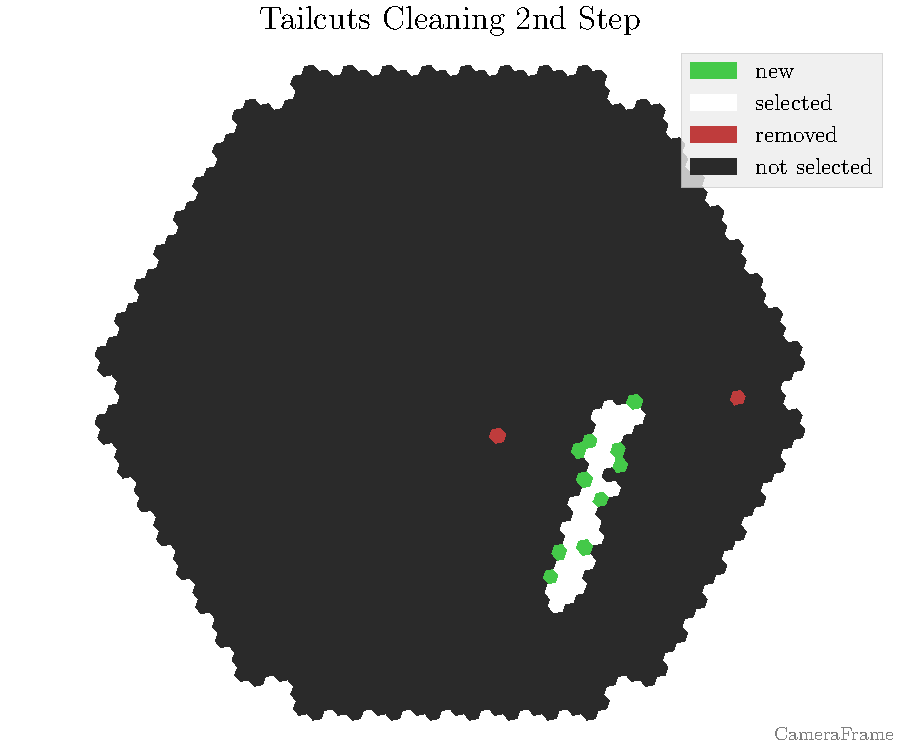
\includegraphics[width=\textwidth]{plots/cleaner_steps/light/tail_2.pdf}
      }
      \only<6>{
      \begin{itemize}
        \setlength\itemsep{1em}
        \item \code{darkgray!50!white}{TailcutsImageCleaner}
        \item \code{darkgray}{MARSImageCleaner}
        \item \code{darkgray!50!white}{FACTImageCleaner}
        \item \code{darkgray!50!white}{TimeConstrainedImageCleaner}
      \end{itemize}
      }
      \only<7>{
        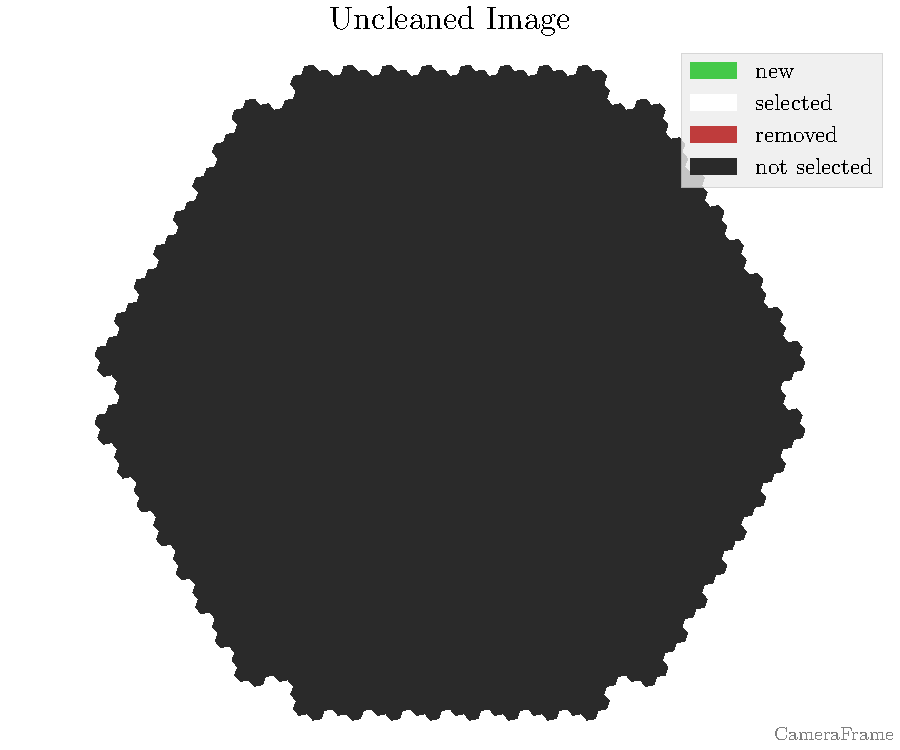
\includegraphics[width=\textwidth]{plots/cleaner_steps/light/null_image.pdf}
      }
      \only<8>{
        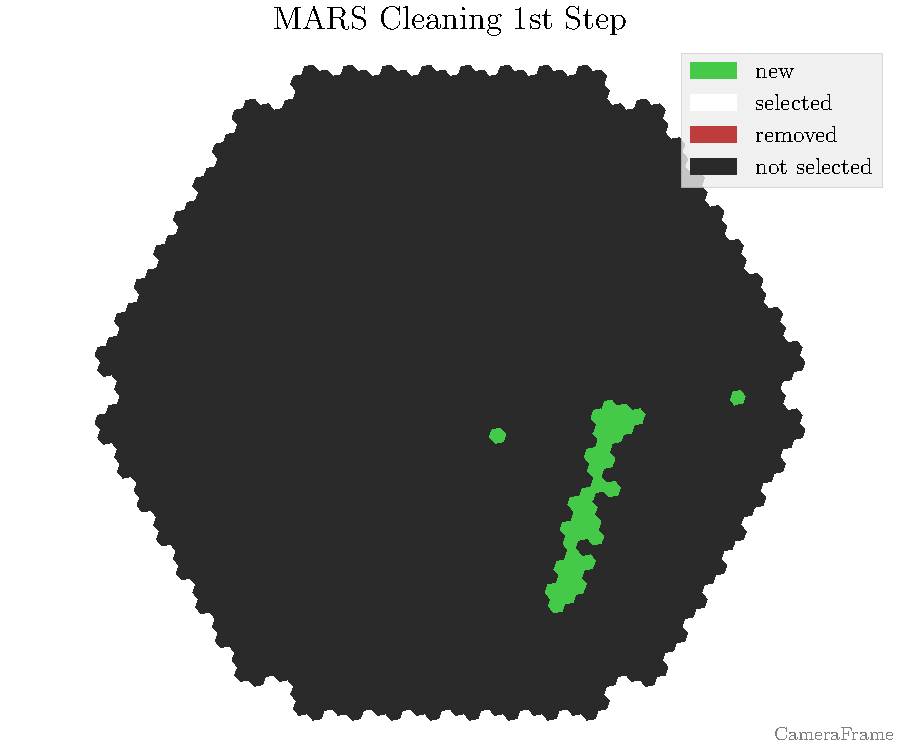
\includegraphics[width=\textwidth]{plots/cleaner_steps/light/mars_1.pdf}
      }
      \only<9>{
        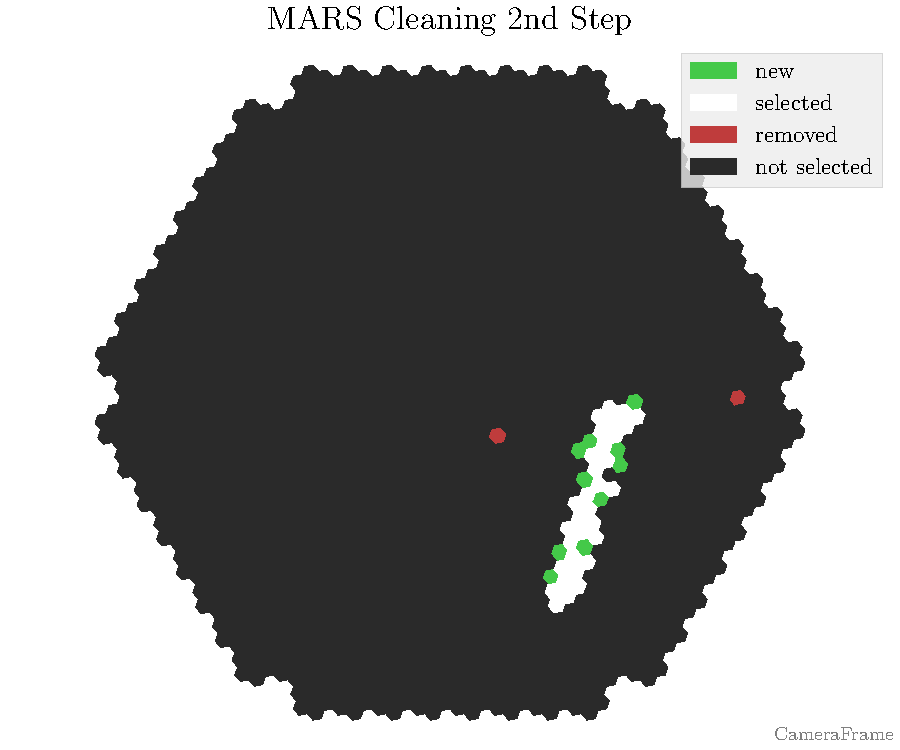
\includegraphics[width=\textwidth]{plots/cleaner_steps/light/mars_2.pdf}
      }
      \only<10>{
        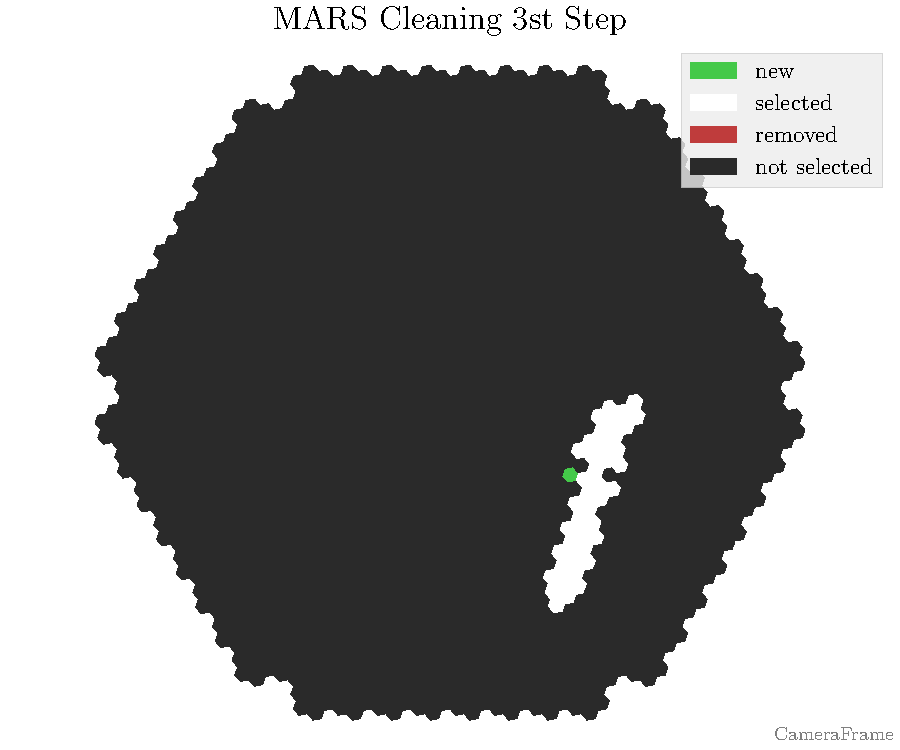
\includegraphics[width=\textwidth]{plots/cleaner_steps/light/mars_3.pdf}
      }
      \only<11>{
      \begin{itemize}
        \setlength\itemsep{1em}
        \item \code{darkgray!50!white}{TailcutsImageCleaner}
        \item \code{darkgray!50!white}{MARSImageCleaner}
        \item \code{darkgray}{FACTImageCleaner}
        \item \code{darkgray!50!white}{TimeConstrainedImageCleaner}
      \end{itemize}
      }
      \only<12>{
        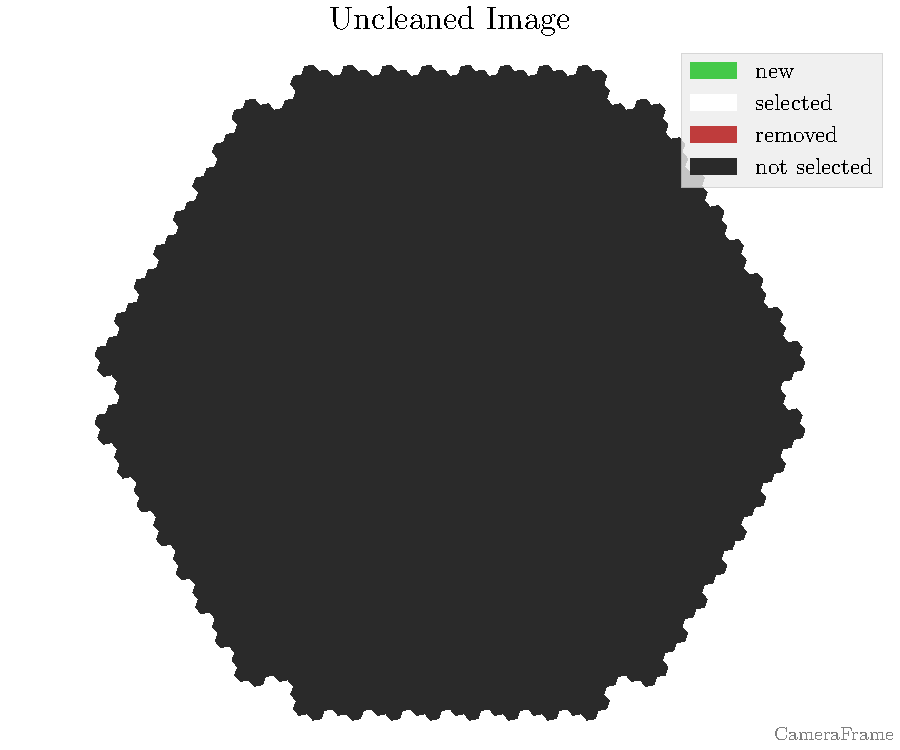
\includegraphics[width=\textwidth]{plots/cleaner_steps/light/null_image.pdf}
      }
      \only<13>{
        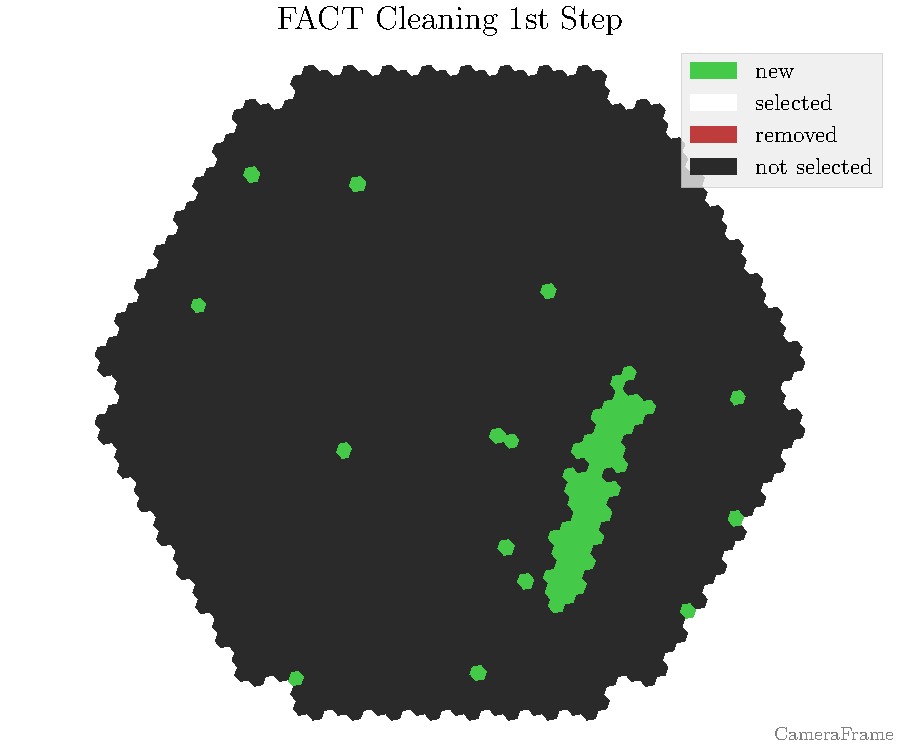
\includegraphics[width=\textwidth]{plots/cleaner_steps/light/fact_1.pdf}
      }
      \only<14>{
        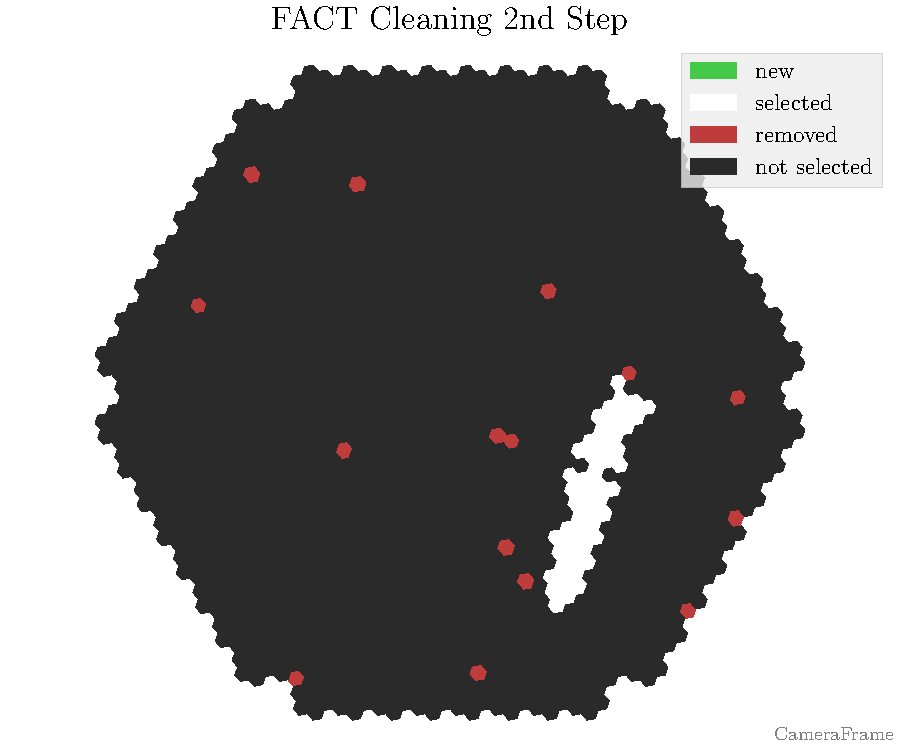
\includegraphics[width=\textwidth]{plots/cleaner_steps/light/fact_2.pdf}
      }
      \only<15>{
        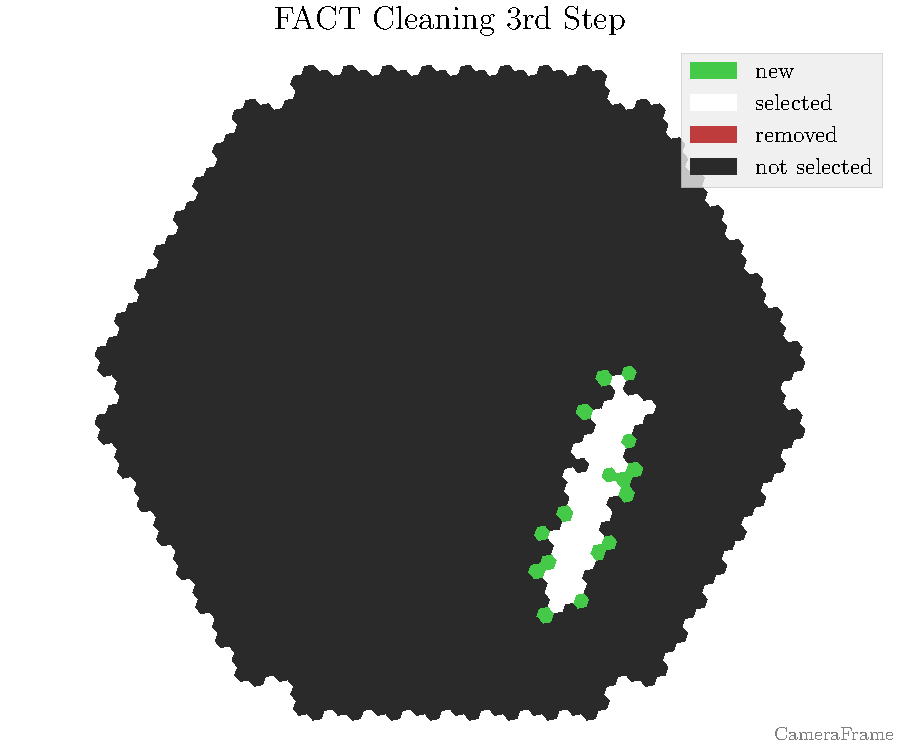
\includegraphics[width=\textwidth]{plots/cleaner_steps/light/fact_3.pdf}
      }
      \only<16>{
        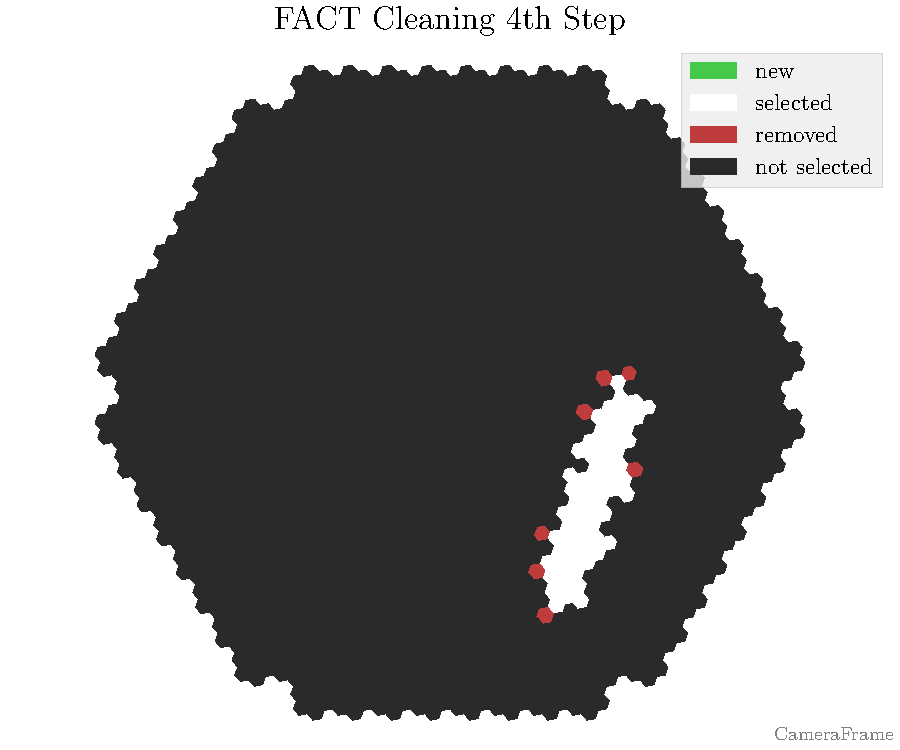
\includegraphics[width=\textwidth]{plots/cleaner_steps/light/fact_4.pdf}
      }
      \only<17>{
        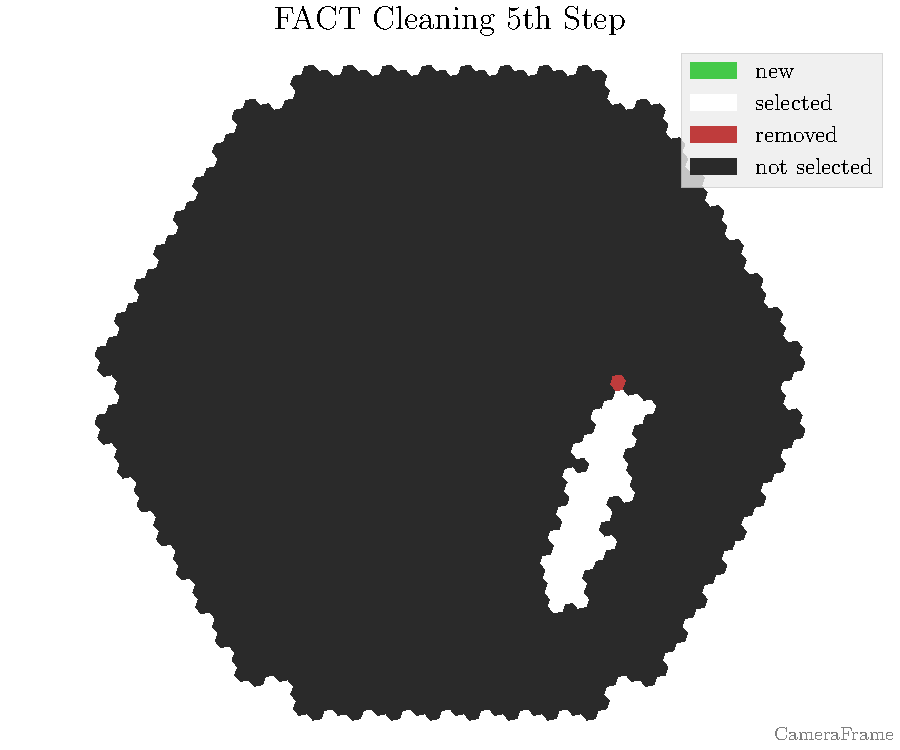
\includegraphics[width=\textwidth]{plots/cleaner_steps/light/fact_5.pdf}
      }
      \only<18>{
        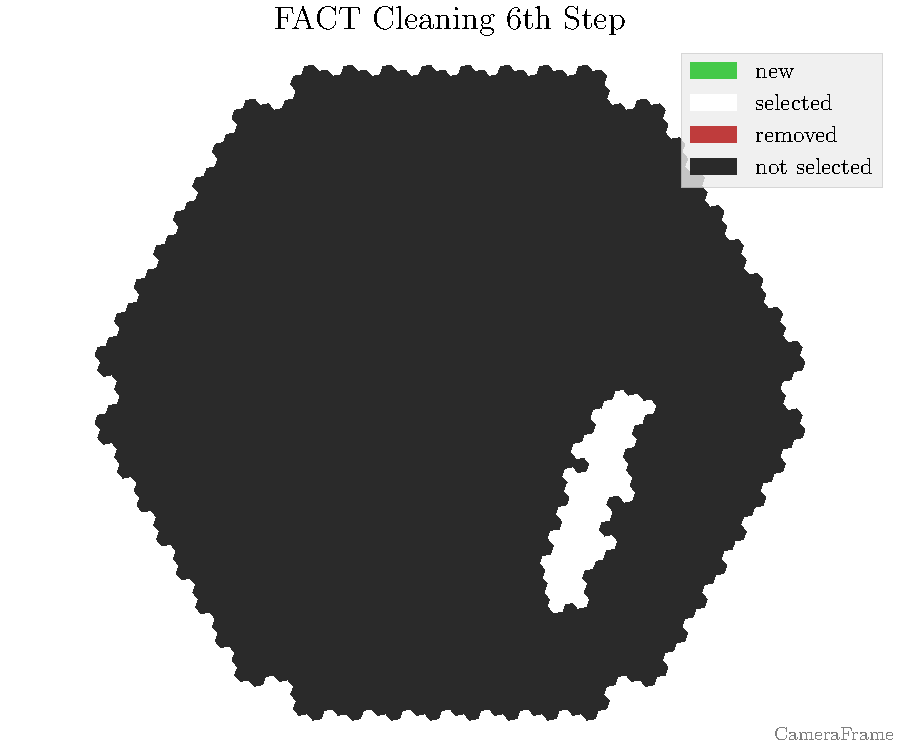
\includegraphics[width=\textwidth]{plots/cleaner_steps/light/fact_6.pdf}
      }
      \only<19>{
      \begin{itemize}
        \setlength\itemsep{1em}
        \item \code{darkgray!50!white}{TailcutsImageCleaner}
        \item \code{darkgray!50!white}{MARSImageCleaner}
        \item \code{darkgray!50!white}{FACTImageCleaner}
        \item \code{darkgray}{TimeConstrainedImageCleaner}
      \end{itemize}
      }
      \only<20>{
        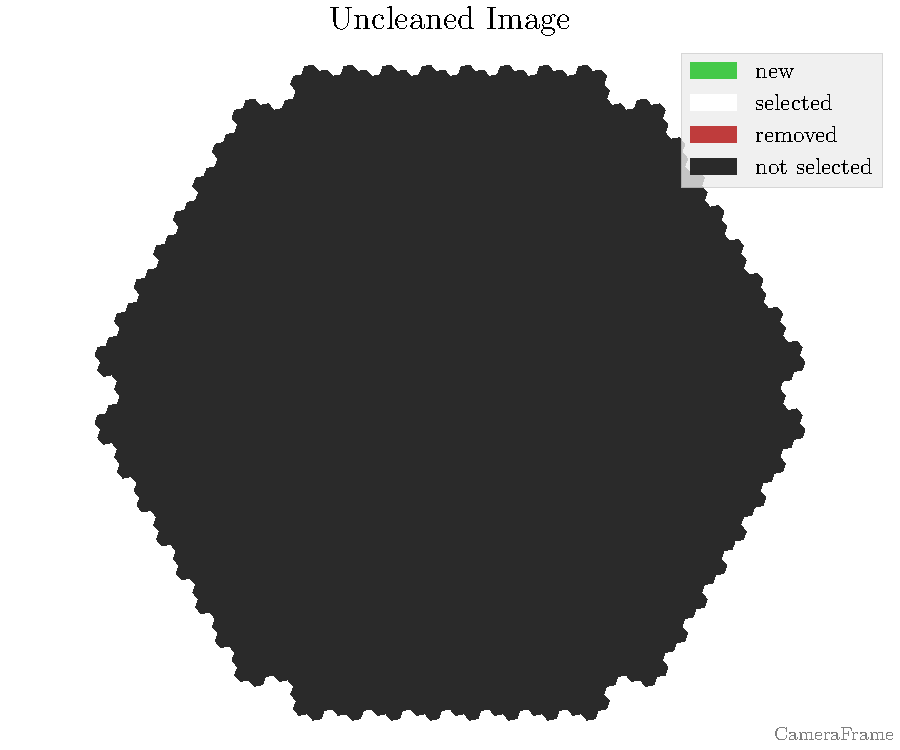
\includegraphics[width=\textwidth]{plots/cleaner_steps/light/null_image.pdf}
      }
      \only<21>{
        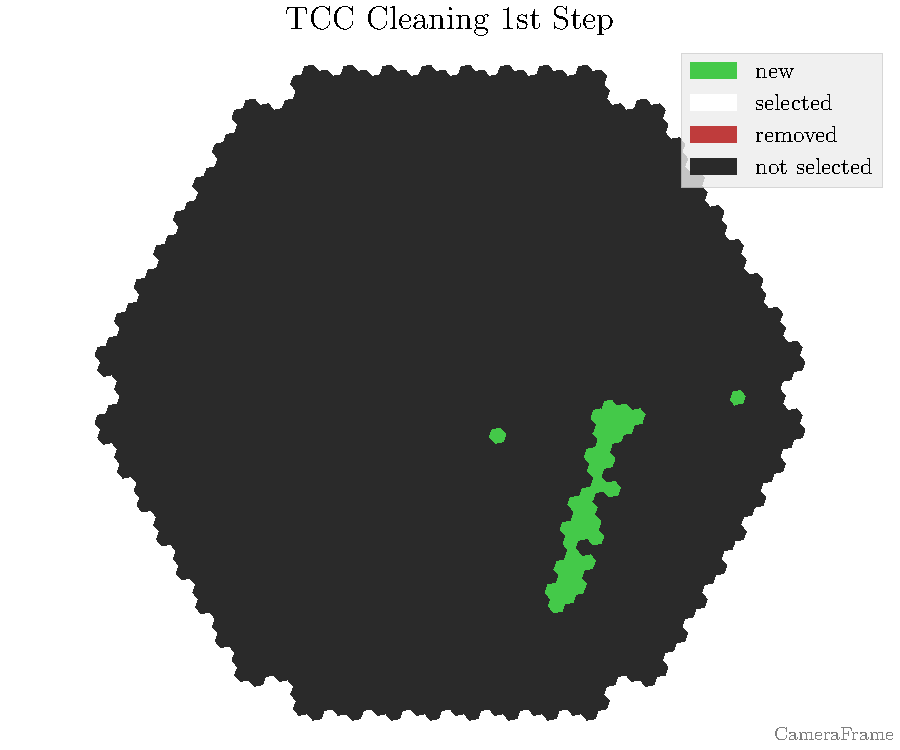
\includegraphics[width=\textwidth]{plots/cleaner_steps/light/tcc_1.pdf}
      }
      \only<22>{
        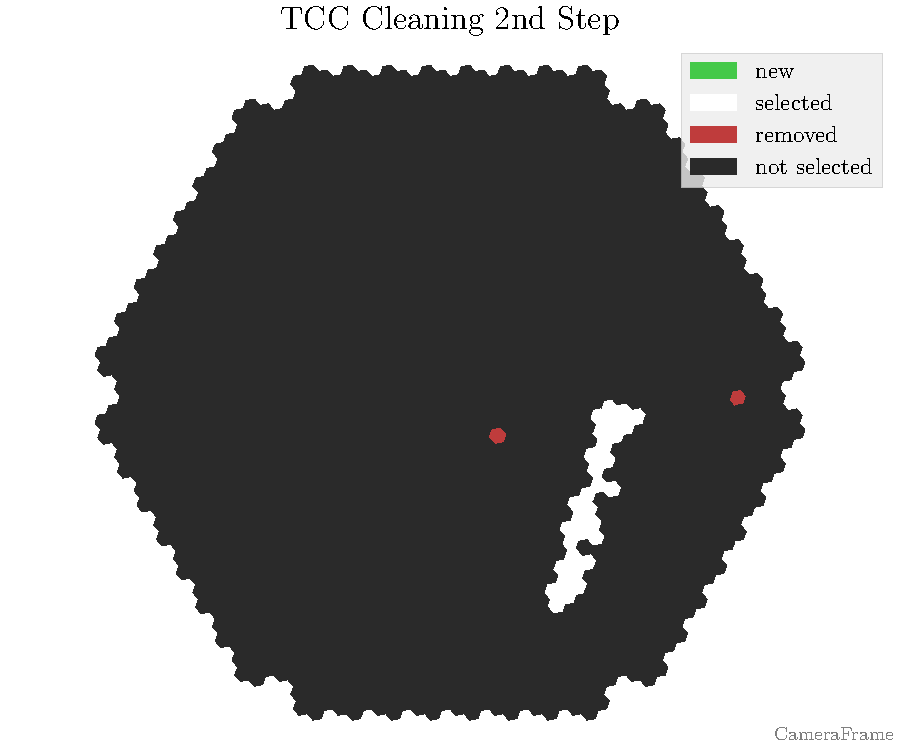
\includegraphics[width=\textwidth]{plots/cleaner_steps/light/tcc_2.pdf}
      }
      \only<23>{
        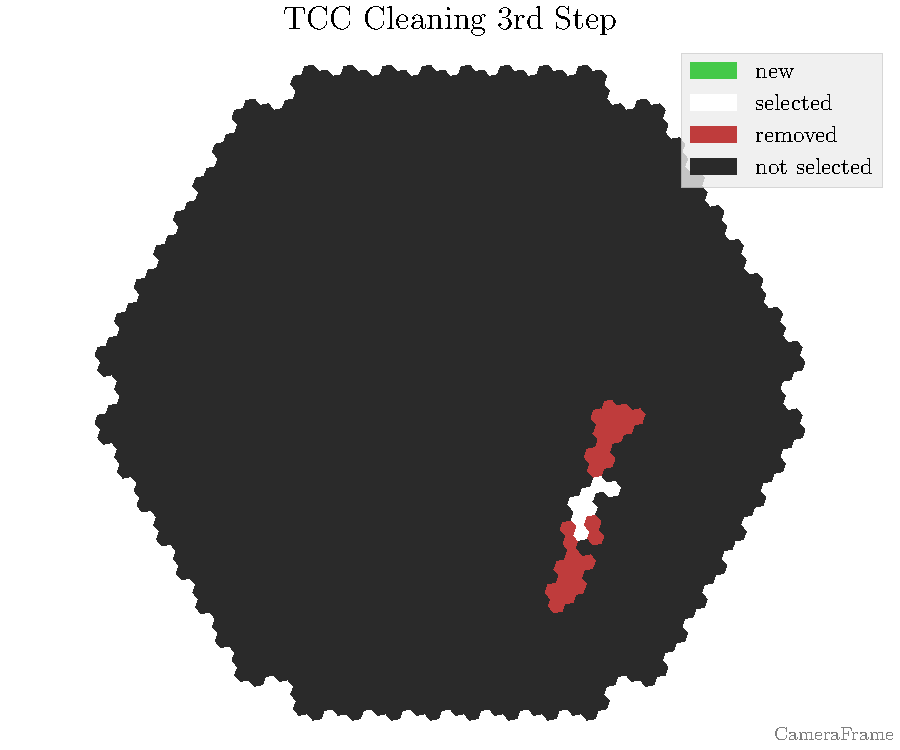
\includegraphics[width=\textwidth]{plots/cleaner_steps/light/tcc_3.pdf}
      }
      \only<24>{
        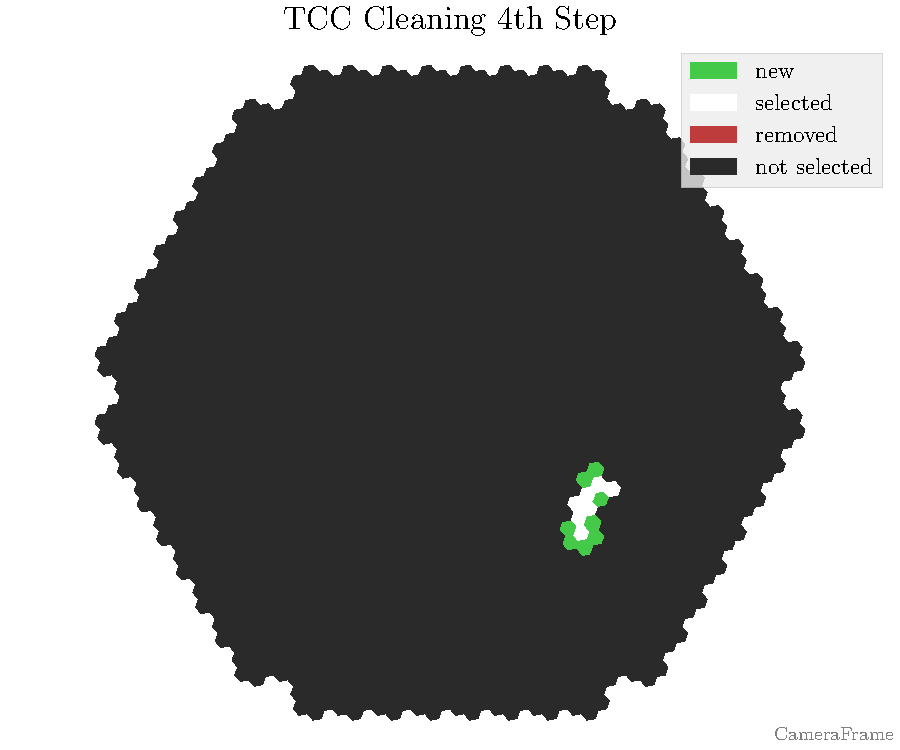
\includegraphics[width=\textwidth]{plots/cleaner_steps/light/tcc_4.pdf}
      }
      \only<25>{
        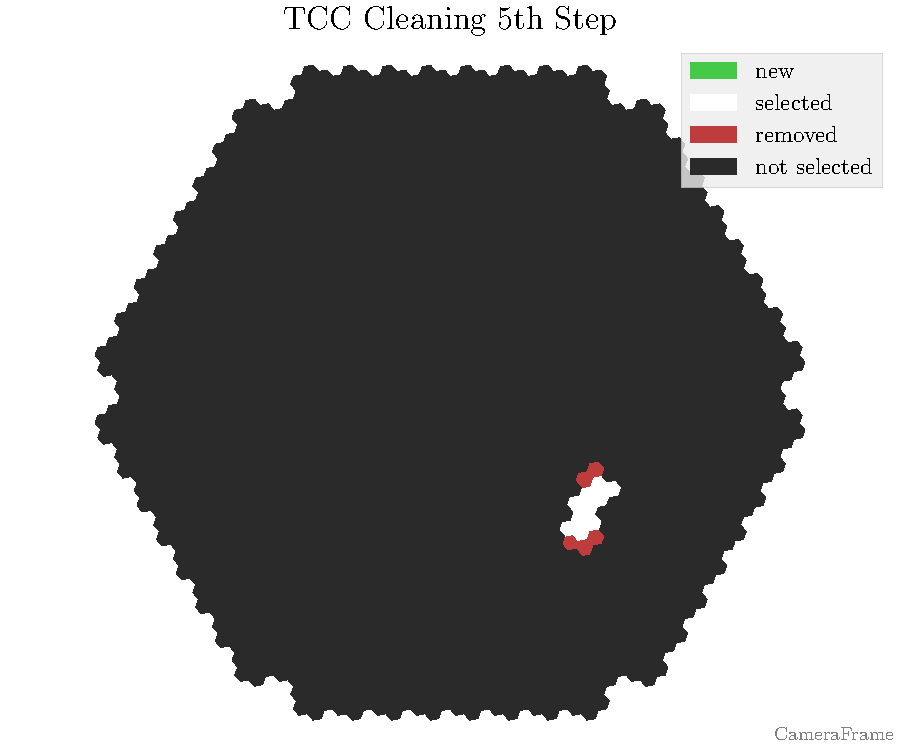
\includegraphics[width=\textwidth]{plots/cleaner_steps/light/tcc_5.pdf}
      }
    \end{overlayarea}
    }
    \raisebox{10ex}{
    \begin{overlayarea}{0.58\textwidth}{3.5cm}
      \only<1>{
        \centering
        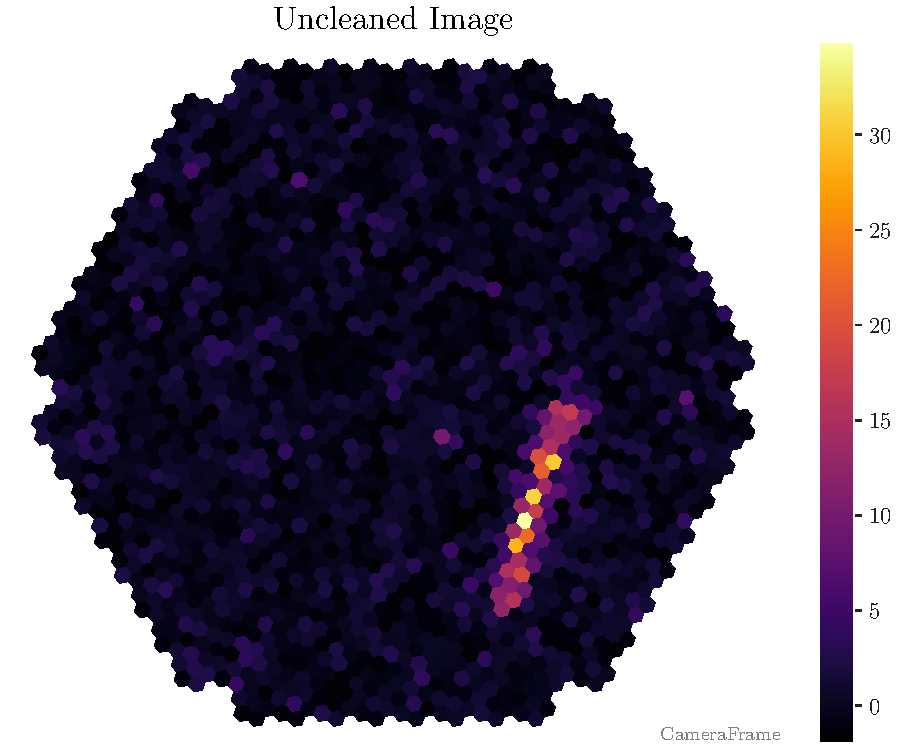
\includegraphics[width=0.65\textwidth]{plots/cleaner_steps/light/uncleaned_image.pdf}
      }
      \only<2>{
      \begin{enumerate}%TailcutsImageCleaner
        \item Select pixels that pass the \code{darkgray!70!white}{core threshold} (this talk: \(\SI{7}{\pe}\))
        \item Add pixels that pass the \code{darkgray!70!white}{boundary threshold} (here: \(\SI{5}{\pe}\))
      \end{enumerate}
      }
      \only<3>{
      \begin{enumerate}%TailcutsImageCleaner
        \item \textcolor{darkgray!50!white}{Select pixels that pass the \code{darkgray!35!white}{core threshold} (this talk: \(\SI{7}{\pe}\))}
        \item \textcolor{darkgray!50!white}{Add pixels that pass the \code{darkgray!35!white}{boundary threshold} (here: \(\SI{5}{\pe}\))}
      \end{enumerate}
      }
      \only<4>{
      \begin{enumerate}%TailcutsImageCleaner
        \item Select pixels that pass the \code{darkgray!70!white}{core threshold} (this talk: \(\SI{7}{\pe}\))
        \item \textcolor{darkgray!50!white}{Add pixels that pass the \code{darkgray!35!white}{boundary threshold} (here: \(\SI{5}{\pe}\))}
      \end{enumerate}
      }
      \only<5>{
      \begin{enumerate}%TailcutsImageCleaner
        \item \textcolor{darkgray!50!white}{Select pixels that pass the \code{darkgray!35!white}{core threshold} (this talk: \(\SI{7}{\pe}\))}
        \item Add pixels that pass the \code{darkgray!70!white}{boundary threshold} (here: \(\SI{5}{\pe}\))
      \end{enumerate}
      }

      \only<6>{
      \begin{enumerate}%MARSImageCleaner
        \item Select pixels that pass the \code{darkgray!70!white}{core} and \code{darkgray!70!white}{boundary threshold}, analogous to \code{darkgray!70!white}{TailcutsImageCleaner}
        \item Add pixels that are a neighbor of a neighbor of a core pixel, if they are above the \code{darkgray!70!white}{boundary threshold}
      \end{enumerate}
      }
      \only<7>{
      \begin{enumerate}%MARSImageCleaner
        \item \textcolor{darkgray!50!white}{Select pixels that pass the \code{darkgray!35!white}{core} and \code{darkgray!35!white}{boundary threshold}, analogous to \code{darkgray!35!white}{TailcutsImageCleaner}}
        \item \textcolor{darkgray!50!white}{Add pixels that are a neighbor of a neighbor of a core pixel, if they are above the \code{darkgray!35!white}{boundary threshold}}
      \end{enumerate}
      }
      \only<8-9>{
      \begin{enumerate}%MARSImageCleaner
        \item Select pixels that pass the \code{darkgray!70!white}{core} and \code{darkgray!70!white}{boundary threshold}, analogous to \code{darkgray!70!white}{TailcutsImageCleaner}
        \item \textcolor{darkgray!50!white}{Add pixels that are a neighbor of a neighbor of a core pixel, if they are above the \code{darkgray!35!white}{boundary threshold}}
      \end{enumerate}
      }
      \only<10>{
      \begin{enumerate}%MARSImageCleaner
        \item \textcolor{darkgray!50!white}{Select pixels that pass the \code{darkgray!35!white}{core} and \code{darkgray!35!white}{boundary threshold}, analogous to \code{darkgray!35!white}{TailcutsImageCleaner}}
        \item Add pixels that are a neighbor of a neighbor of a core pixel, if they are above the \code{darkgray!70!white}{boundary threshold}
      \end{enumerate}
      }
      \only<11>{
      \begin{enumerate}%FACTImageCleaner
        \item Find all pixels that contain more photons than the \code{darkgray!70!white}{core threshold} (this talk: \(\SI{4}{\pe}\))
        \item Remove pixels with less than \(N\) neighbors (this talk: \(N=2\))
        \item Add remaining neighbors that are above the \code{darkgray!70!white}{boundary threshold} (this talk: \(\SI{2}{\pe}\))
        \item Remove pixels that have less than \(N\) neighbors, that arrive within a given timeframe (here: \SI{5}{\nano\second})
        \item Remove pixels that have less than \(N\) neighbors
        \item Remove pixels that have less than \(N\) neighbors, arriving within a given timeframe (same as in step 4)
      \end{enumerate}
      }
      \only<12>{
      \begin{enumerate}%FACTImageCleaner
        \item \textcolor{darkgray!50!white}{Find all pixels that contain more photons than the \code{darkgray!35!white}{core threshold} (this talk: \(\SI{4}{\pe}\))}
        \item \textcolor{darkgray!50!white}{Remove pixels with less than \(N\) neighbors (this talk: \(N=2\))}
        \item \textcolor{darkgray!50!white}{Add remaining neighbors that are above the \code{darkgray!35!white}{boundary threshold} (this talk: \(\SI{2}{\pe}\))}
        \item \textcolor{darkgray!50!white}{Remove pixels that have less than \(N\) neighbors, that arrive within a given timeframe (here: \SI{5}{\nano\second})}
        \item \textcolor{darkgray!50!white}{Remove pixels that have less than \(N\) neighbors}
        \item \textcolor{darkgray!50!white}{Remove pixels that have less than \(N\) neighbors, arriving within a given timeframe (same as in step 4)}
      \end{enumerate}
      }
      \only<13>{
      \begin{enumerate}%FACTImageCleaner
        \item Find all pixels that contain more photons than the \code{darkgray!70!white}{core threshold} (this talk: \(\SI{4}{\pe}\))
        \item \textcolor{darkgray!50!white}{Remove pixels with less than \(N\) neighbors (this talk: \(N=2\))}
        \item \textcolor{darkgray!50!white}{Add remaining neighbors that are above the \code{darkgray!35!white}{boundary threshold} (this talk: \(\SI{2}{\pe}\))}
        \item \textcolor{darkgray!50!white}{Remove pixels that have less than \(N\) neighbors, that arrive within a given timeframe (here: \SI{5}{\nano\second})}
        \item \textcolor{darkgray!50!white}{Remove pixels that have less than \(N\) neighbors}
        \item \textcolor{darkgray!50!white}{Remove pixels that have less than \(N\) neighbors, arriving within a given timeframe (same as in step 4)}
      \end{enumerate}
      }
      \only<14>{
      \begin{enumerate}%FACTImageCleaner
        \item \textcolor{darkgray!50!white}{Find all pixels that contain more photons than the \code{darkgray!35!white}{core threshold} (this talk: \(\SI{4}{\pe}\))}
        \item Remove pixels with less than \(N\) neighbors (this talk: \(N=2\))
        \item \textcolor{darkgray!50!white}{Add remaining neighbors that are above the \code{darkgray!35!white}{boundary threshold} (this talk: \(\SI{2}{\pe}\))}
        \item \textcolor{darkgray!50!white}{Remove pixels that have less than \(N\) neighbors, that arrive within a given timeframe (here: \SI{5}{\nano\second})}
        \item \textcolor{darkgray!50!white}{Remove pixels that have less than \(N\) neighbors}
        \item \textcolor{darkgray!50!white}{Remove pixels that have less than \(N\) neighbors, arriving within a given timeframe (same as in step 4)}
      \end{enumerate}
      }
      \only<15>{
      \begin{enumerate}%FACTImageCleaner
        \item \textcolor{darkgray!50!white}{Find all pixels that contain more photons than the \code{darkgray!35!white}{core threshold} (this talk: \(\SI{4}{\pe}\))}
        \item \textcolor{darkgray!50!white}{Remove pixels with less than \(N\) neighbors (this talk: \(N=2\))}
        \item Add remaining neighbors that are above the \code{darkgray!70!white}{boundary threshold} (this talk: \(\SI{2}{\pe}\))
        \item \textcolor{darkgray!50!white}{Remove pixels that have less than \(N\) neighbors, that arrive within a given timeframe (here: \SI{5}{\nano\second})}
        \item \textcolor{darkgray!50!white}{Remove pixels that have less than \(N\) neighbors}
        \item \textcolor{darkgray!50!white}{Remove pixels that have less than \(N\) neighbors, arriving within a given timeframe (same as in step 4)}
      \end{enumerate}
      }
      \only<16>{
      \begin{enumerate}%FACTImageCleaner
        \item \textcolor{darkgray!50!white}{Find all pixels that contain more photons than the \code{darkgray!35!white}{core threshold} (this talk: \(\SI{4}{\pe}\))}
        \item \textcolor{darkgray!50!white}{Remove pixels with less than \(N\) neighbors (this talk: \(N=2\))}
        \item \textcolor{darkgray!50!white}{Add remaining neighbors that are above the \code{darkgray!35!white}{boundary threshold} (this talk: \(\SI{2}{\pe}\))}
        \item Remove pixels that have less than \(N\) neighbors, that arrive within a given timeframe (here: \SI{5}{\nano\second})
        \item \textcolor{darkgray!50!white}{Remove pixels that have less than \(N\) neighbors}
        \item \textcolor{darkgray!50!white}{Remove pixels that have less than \(N\) neighbors, arriving within a given timeframe (same as in step 4)}
      \end{enumerate}
      }
      \only<17>{
      \begin{enumerate}%FACTImageCleaner
        \item \textcolor{darkgray!50!white}{Find all pixels that contain more photons than the \code{darkgray!35!white}{core threshold} (this talk: \(\SI{4}{\pe}\))}
        \item \textcolor{darkgray!50!white}{Remove pixels with less than \(N\) neighbors (this talk: \(N=2\))}
        \item \textcolor{darkgray!50!white}{Add remaining neighbors that are above the \code{darkgray!35!white}{boundary threshold} (this talk: \(\SI{2}{\pe}\))}
        \item \textcolor{darkgray!50!white}{Remove pixels that have less than \(N\) neighbors, that arrive within a given timeframe (here: \SI{5}{\nano\second})}
        \item Remove pixels that have less than \(N\) neighbors
        \item \textcolor{darkgray!50!white}{Remove pixels that have less than \(N\) neighbors, arriving within a given timeframe (same as in step 4)}
      \end{enumerate}
      }
      \only<18>{
      \begin{enumerate}%FACTImageCleaner
        \item \textcolor{darkgray!50!white}{Find all pixels that contain more photons than the \code{darkgray!35!white}{core threshold} (this talk: \(\SI{4}{\pe}\))}
        \item \textcolor{darkgray!50!white}{Remove pixels with less than \(N\) neighbors (this talk: \(N=2\))}
        \item \textcolor{darkgray!50!white}{Add remaining neighbors that are above the \code{darkgray!35!white}{boundary threshold} (this talk: \(\SI{2}{\pe}\))}
        \item \textcolor{darkgray!50!white}{Remove pixels that have less than \(N\) neighbors, that arrive within a given timeframe (here: \SI{5}{\nano\second})}
        \item \textcolor{darkgray!50!white}{Remove pixels that have less than \(N\) neighbors}
        \item Remove pixels that have less than \(N\) neighbors, arriving within the given timeframe (same as in step 4)
      \end{enumerate}
      }
      \only<19>{
      \begin{enumerate}%TimeConstrainedImageCleaner
        \item Find all core pixels above the \code{darkgray!70!white}{core threshold} (this talk: \(\SI{7}{\pe}\))
        \item Remove pixels with less than \(N\) neighbors (this talk: \(N=1\))
        \item Keep all pixels that arrive within a time limit of the average arrival time (\code{darkgray!70!white}{time_limit_core}: \SI{4.5}{\nano\second})
        \item Find all neighboring pixels above the \code{darkgray!70!white}{boundary threshold} (this talk: \(\SI{5}{\pe}\))
        \item Remove all pixels with less than \(N\) neighbors arriving within a given timeframe (\code{darkgray!70!white}{time_limit_boundary}: \SI{1.5}{\nano\second})
      \end{enumerate}
      }
      \only<20>{
      \begin{enumerate}%TimeConstrainedImageCleaner
        \item \textcolor{darkgray!50!white}{Find all core pixels above the \code{darkgray!35!white}{core threshold} (this talk: \(\SI{7}{\pe}\))}
        \item \textcolor{darkgray!50!white}{Remove pixels with less than \(N\) neighbors (this talk: \(N=1\))}
        \item \textcolor{darkgray!50!white}{Keep all pixels that arrive within a time limit of the average arrival time (\code{darkgray!35!white}{time_limit_core}: \SI{4.5}{\nano\second})}
        \item \textcolor{darkgray!50!white}{Find all neighboring pixels above the \code{darkgray!35!white}{boundary threshold} (this talk: \(\SI{5}{\pe}\))}
        \item \textcolor{darkgray!50!white}{Remove all pixels with less than \(N\) neighbors arriving within a given timeframe (\code{darkgray!35!white}{time_limit_boundary}: \SI{1.5}{\nano\second})}
      \end{enumerate}
      }
      \only<21>{
      \begin{enumerate}%TimeConstrainedImageCleaner
        \item Find all core pixels above the \code{darkgray!70!white}{core threshold} (this talk: \(\SI{7}{\pe}\))
        \item \textcolor{darkgray!50!white}{Remove pixels with less than \(N\) neighbors (this talk: \(N=1\))}
        \item \textcolor{darkgray!50!white}{Keep all pixels that arrive within a time limit of the average arrival time (\code{darkgray!35!white}{time_limit_core}: \SI{4.5}{\nano\second})}
        \item \textcolor{darkgray!50!white}{Find all neighboring pixels above the \code{darkgray!35!white}{boundary threshold} (this talk: \(\SI{5}{\pe}\))}
        \item \textcolor{darkgray!50!white}{Remove all pixels with less than \(N\) neighbors arriving within a given timeframe (\code{darkgray!35!white}{time_limit_boundary}: \SI{1.5}{\nano\second})}
      \end{enumerate}
      }
      \only<22>{
      \begin{enumerate}%TimeConstrainedImageCleaner
        \item \textcolor{darkgray!50!white}{Find all core pixels above the \code{darkgray!35!white}{core threshold} (this talk: \(\SI{7}{\pe}\))}
        \item Remove pixels with less than \(N\) neighbors (this talk: \(N=1\))
        \item \textcolor{darkgray!50!white}{Keep all pixels that arrive within a time limit of the average arrival time (\code{darkgray!35!white}{time_limit_core}: \SI{4.5}{\nano\second})}
        \item \textcolor{darkgray!50!white}{Find all neighboring pixels above the \code{darkgray!35!white}{boundary threshold} (this talk: \(\SI{5}{\pe}\))}
        \item \textcolor{darkgray!50!white}{Remove all pixels with less than \(N\) neighbors arriving within a given timeframe (\code{darkgray!35!white}{time_limit_boundary}: \SI{1.5}{\nano\second})}
      \end{enumerate}
      }
      \only<23>{
      \begin{enumerate}%TimeConstrainedImageCleaner
        \item \textcolor{darkgray!50!white}{Find all core pixels above the \code{darkgray!35!white}{core threshold} (this talk: \(\SI{7}{\pe}\))}
        \item \textcolor{darkgray!50!white}{Remove pixels with less than \(N\) neighbors (this talk: \(N=1\))}
        \item Keep all pixels that arrive within a time limit of the average arrival time (\code{darkgray!70!white}{time_limit_core}: \SI{4.5}{\nano\second})
        \item \textcolor{darkgray!50!white}{Find all neighboring pixels above the \code{darkgray!35!white}{boundary threshold} (this talk: \(\SI{5}{\pe}\))}
        \item \textcolor{darkgray!50!white}{Remove all pixels with less than \(N\) neighbors arriving within a given timeframe (\code{darkgray!35!white}{time_limit_boundary}: \SI{1.5}{\nano\second})}
      \end{enumerate}
      }
      \only<24>{
      \begin{enumerate}%TimeConstrainedImageCleaner
        \item \textcolor{darkgray!50!white}{Find all core pixels above the \code{darkgray!35!white}{core threshold} (this talk: \(\SI{7}{\pe}\))}
        \item \textcolor{darkgray!50!white}{Remove pixels with less than \(N\) neighbors (this talk: \(N=1\))}
        \item \textcolor{darkgray!50!white}{Keep all pixels that arrive within a time limit of the average arrival time (\code{darkgray!35!white}{time_limit_core}: \SI{4.5}{\nano\second})}
        \item Find all neighboring pixels above the \code{darkgray!70!white}{boundary threshold} (this talk: \(\SI{5}{\pe}\))
        \item \textcolor{darkgray!50!white}{Remove all pixels with less than \(N\) neighbors arriving within a given timeframe (\code{darkgray!35!white}{time_limit_boundary}: \SI{1.5}{\nano\second})}
      \end{enumerate}
      }
      \only<25>{
      \begin{enumerate}%TimeConstrainedImageCleaner
        \item \textcolor{darkgray!50!white}{Find all core pixels above the \code{darkgray!35!white}{core threshold} (this talk: \(\SI{7}{\pe}\))}
        \item \textcolor{darkgray!50!white}{Remove pixels with less than \(N\) neighbors (this talk: \(N=1\))}
        \item \textcolor{darkgray!50!white}{Keep all pixels that arrive within a time limit of the average arrival time (\code{darkgray!35!white}{time_limit_core}: \SI{4.5}{\nano\second})}
        \item \textcolor{darkgray!50!white}{Find all neighboring pixels above the \code{darkgray!35!white}{boundary threshold} (this talk: \(\SI{5}{\pe}\))}
        \item Remove all pixels with less than \(N\) neighbors arriving within a given timeframe (\code{darkgray!70!white}{time_limit_boundary}: \SI{1.5}{\nano\second})
      \end{enumerate}
      }
    \end{overlayarea}
    }
  \end{frame}
    }

\subsection{Hyperparameters}%
\label{sub:Hyperparameters}
\begin{frame}{Selecting reasonable hyperparameters for the grid search}
    % \todo[inline]{might need to think more about the layout of this slide}
    \begin{overlayarea}{\textwidth}{2.5cm}
        \begin{itemize}
            \item<1-> Begin by calculating core thresholds from quantiles for a given telescope type
            \item<3-> Select the boundary thresholds as ratios of the core thresholds (\eg 0.25, 0.33, 0.5\dots)
            \item<4-> Select feasible values for the number of neighbors (\eg 0, 1, 2, 3,\dots)
            \item<5-> Set reasonable time limits for the time-based algorithms
        \end{itemize}
        % \vspace{0.5cm}
    \end{overlayarea}
    \begin{overlayarea}{\textwidth}{\textheight}
        \only<2->{
            \ifthenelse{\equal{\theme}{\string 1}}
            {% use dark theme
            \vfill
            \centering
            \includegraphics[width=0.85\textwidth]{build/quantiles_plot_dark.pdf}
            }
            {% use light theme
            \vfill
            \centering
            \includegraphics[width=0.85\textwidth]{build/quantiles_plot_light.pdf}
            }
        }
    \end{overlayarea}
\end{frame}